\documentclass[10pt,portrait, twocolumn]{article}
\usepackage{multicol}
\usepackage{calc}
\usepackage[portrait]{geometry}
\usepackage{amsmath,amsthm,amsfonts,amssymb}
\usepackage{times}
\usepackage{color,graphicx,overpic}
\graphicspath{ {images/} }
\usepackage{hyperref}
\usepackage{pgfplots}
\usepackage{esint}
\usepackage{bm}
\usepackage{tikz}
\usepackage{relsize}
\usepackage{datetime}
\usepackage[utf8] {inputenc}
\usepackage[spanish, activeacute] {babel}
\usepackage{IEEEtrantools}
\usepackage{color}

\usepackage{framed}

\usepackage{pdflscape}

%\usepackage{draftwatermark}
%\SetWatermarkText{Javier de Martín}
%\SetWatermarkScale{0.8}

% This sets page margins to .5 inch if using letter paper, and to 1cm
% if using A4 paper. (This probably isn't strictly necessary.)
% If using another size paper, use default 1cm margins.
\geometry{top=.5cm,left=.5cm,right=.5cm,bottom=.5cm}
    
\pgfplotsset{
    dirac/.style={
        mark=triangle*,
        mark options={scale=2},
        ycomb,
        scatter,
        visualization depends on={y/abs(y)-1 \as \sign},
        scatter/@pre marker code/.code={\scope[rotate=90*\sign,yshift=-2pt]}
    }
}

% Turn off header and footer
\pagestyle{empty}

% Redefine section commands to use less space
\makeatletter
\renewcommand{\section}{\@startsection{section}{1}{0mm}%
                                {-1ex plus -.5ex minus -.2ex}%
                                {0.5ex plus .2ex}%x
                                {\normalfont\large\bfseries}}
\renewcommand{\subsection}{\@startsection{subsection}{2}{0mm}%
                                {-1explus -.5ex minus -.2ex}%
                                {0.5ex plus .2ex}%
                                {\normalfont\normalsize\bfseries}}
\renewcommand{\subsubsection}{\@startsection{subsubsection}{3}{0mm}%
                                {-1ex plus -.5ex minus -.2ex}%
                                {1ex plus .2ex}%
                                {\normalfont\small\bfseries}}
\makeatother

\newcommand{\Lagr}{\mathcal{L}}

% Define BibTeX command
\def\BibTeX{{\rm B\kern-.05em{\sc i\kern-.025em b}\kern-.08em
    T\kern-.1667em\lower.7ex\hbox{E}\kern-.125emX}}

% Don't print section numbers
\setcounter{secnumdepth}{4}


\setlength{\parindent}{0pt}
\setlength{\parskip}{0pt plus 0.5ex}

%My Environments
\newtheorem{example}[section]{Example}
% ---------------------------------------------------------------

\begin{document}


\begin{framed}
	\begin{center}
    	\Large{\underline{Redes de Acceso}} \\
    	\scriptsize{3º Ingeniería de Telecomunicaciones | UPV/EHU}\\
     	%Actualizado por última vez el \today \\
     	"\textsl{Under-promise and over-deliver}." \\
     	%\hspace{5 pt} \\
     	\small{\textbf{Javier de Martín -- 2016/17}}
	\end{center}
\end{framed}

%%%%%%%%%%%%%%%%%%%%%%%%%%%%%%%%%%%%%%%%%%%%%%%%%%%%%%%%%%%%%%%%%


\section{\underline{Introducción}}

Se necesitan redes para la comunicación:

	\begin{itemize}
		\item Sistemas terminales: Terminales y aplicaciones.
		\item Red de Acceso: Red que une el terminal al primer nodo de red.
		\item Núcleo de Red: Conmutación y transmisión.
	\end{itemize}

\subsection{Introducción a las infraestructuras de red. Red de acceso y Red de Transporte}

\subsubsection{Arquitectura General}


\begin{figure}[h]
	\centering
     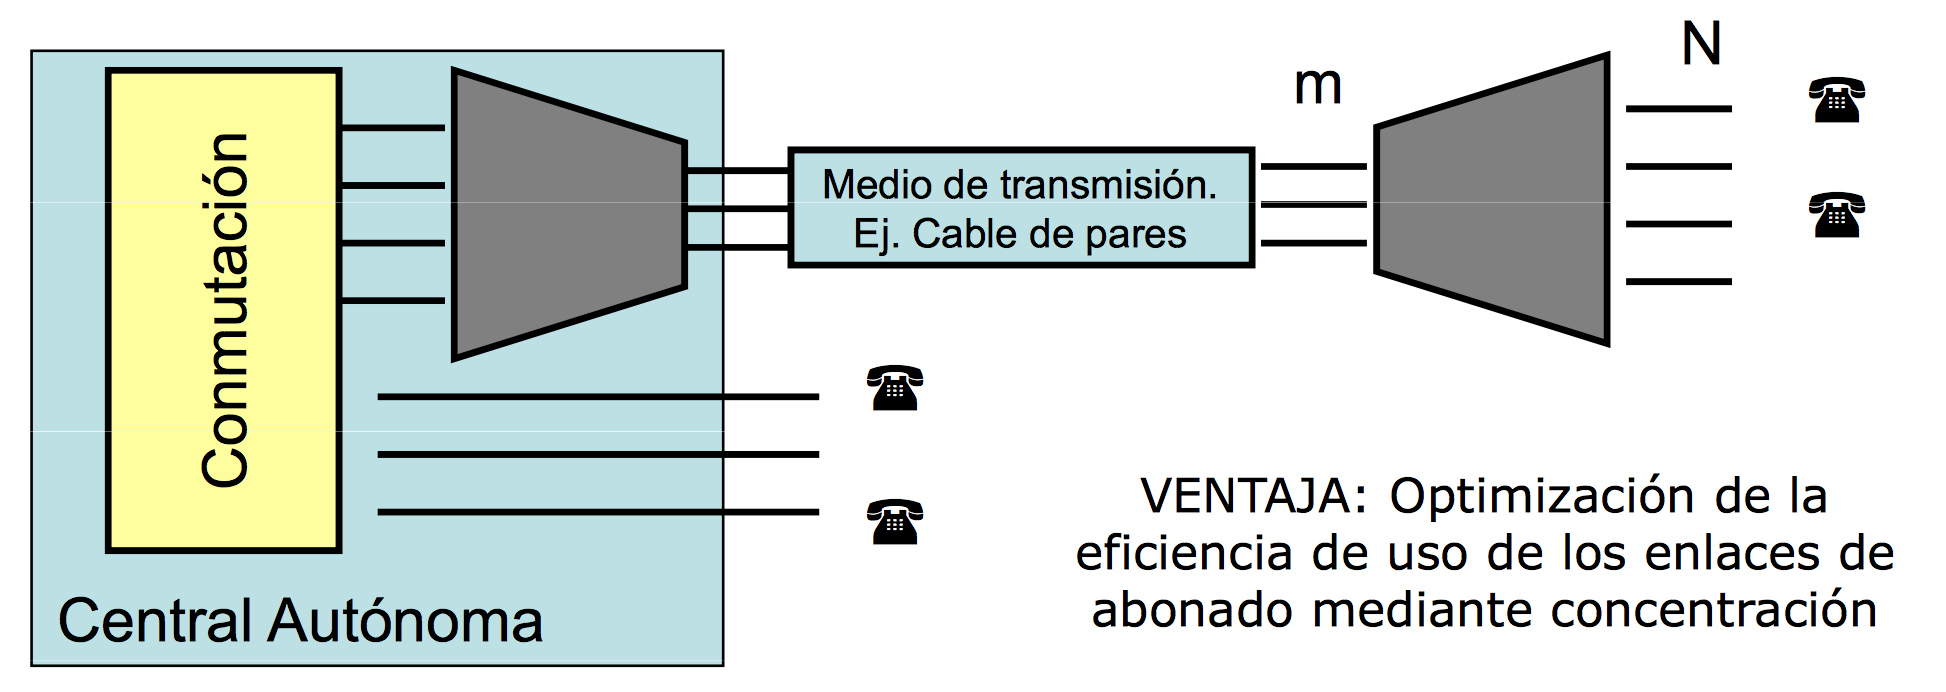
\includegraphics[width=0.35\textwidth]{RedAcceso}
      \caption{Red de acceso}
      \label{fig:ONT}
  \end{figure}
  


La arquitectura de red NGN:
	\begin{itemize}
		\item \textbf{NGN} (\textit{Next Generation Networks}): Red basada en la conmutación de paquetes que permite prestar servicios de telecomunicación y en la que se pueden utilizar múltiples tecnologías de transporte de banda ancha proporcionadas por la QoS, y en la que las funciones relacionadas con los servicios son independientes de las tecnologías subyacentes relacionadas con el transporte. Permite a los usuarios el acceso sin trabas a redes y a proveedores de servicios y/o servicios de su elección. Soporta movilidad generalizada que permitirá la prestación coherente y ubicua de servicios a los usuarios.
		\item \textbf{NGA} (\textit{Next Generation Access}): Describe una importante actualización de la banda ancha disponible, al hacer un cambio de ritmo en la velocidad y calidad del servicio.
	\end{itemize}


\subsubsection{Red de Acceso y Red de Transporte}

La \textbf{red de acceso} es la red existente entre el usuario de un servicio y el primer nodo de servicio que soporta dicho servicio.

\quad La \textbf{red de transporte} proporciona un medio de transmisión entre los nodos de servicio, transportando la información de diferentes servicios de forma conjunta mediante técnicas de multiplexación, y posibilitando la interconexión entre nodos.

\subsubsection{Nodos de Servicio e Interfaces}

Un \textbf{nodo de servicio} es un \textbf{elemento de red} que proporciona acceso a distintos servicios de telecomunicaciones permanentes y/o con conmutación.

\quad Las \textbf{interfaces} unen elementos:

	\begin{itemize}
		\item \textbf{UNI (\textit{User-Network Interface})} $\rightarrow$ Usuario - Red de Acceso. Una misma red de acceso puede dar servicio a diferentes tipos de terminales de usuario, cada uno de ellos con un interfaz distinto. Cada interfaz usuario-red de acceso necesitará unas funciones específicas y una capacidad de servicio de portador determinada. Puede ser individual o compartida.
		\item \textbf{NNI (\textit{Network to Network Interface})} $\rightarrow$ Red de Acceso - Red de Gestión . A través de este interfaz se coordina la operación y mantenimiento de las redes de acceso y red central.
		\item \textbf{SNI (\textit{Service Node Interface})} $\rightarrow$ Red de Acceso - Nodo de Servicio   Los nodos de servicio comparten los recursos de la red de acceso. Plataforma de acceso universal: integración multiservicio. Interfaz abierta: permite desarrollar la red de acceso y el nodo de servicio de forma independiente. Red de acceso es percibida como una subred dividida en múltiples redes de acceso virtuales (una para cada servicio) pero implementadas sobre una misma red física.
		\item Nodo de Servicio - Red de Gestión
	\end{itemize}

\begin{figure}[!ht]
	\centering
     \includegraphics[width=0.35\textwidth]{Frontera}
      \caption{Frontera de la Red de Acceso}
      \label{fig:ONT}
  \end{figure}

\subsection{Introducción a la red de Acceso}

La red de acceso es la realización constituida por entidades como la planta de cables y las facilidades que transmisión que proporcionar las capacidades de portador de transporte requeridas para prestar servicios entre SNIs y UNIs.

\subsubsection{La Red de Acceso}

\textbf{Requerimientos actuales para la red de acceso}, red única que de soporte a todos los servicios con gran ancho de banda y permita movilidad al usuario.

\subsubsection{El Problema de la ``Última Milla'': Despliegue y Cuello de Botella en la Red}

La capacidad de red sigue aumentando exponencialmente y la red de acceso supone un problema y es un cuello de botella. Con las tecnologías de acceso ópticas se proponen nuevas posibilidades.

\subsubsection{Neutralidad de la Red y Calidad de Servicio (QoS)}

La \textbf{neutralidad de la red} es el principio que garantiza el derecho de los usuarios a acceder a cualquier contenido, aplicación o servicio en Internet sin la intervención de los proveedores o censura de la empresas, gobiernos y administraciones. Bajo ese principio, las compañías de telecomunicaciones no podrán filtrar, bloquear, reconducir o favorecer el acceso a unos servicios por encima de otros.\\

El \textbf{efecto de calidad de servicio} determina el grado de satisfacción de un usuario con el servicio. Compromete tanto la calidad de funcionamiento de la red como la calidad de funcionamiento independiente de la red.

\subsection{Arquitecturas de la Red de Acceso}

\subsubsection{Acceso a Redes Públicas - Acceso a Redes Corporativas}

\textbf{Red pública} es toda la red (sin ninguna relación con la situación jurídica del operador de la red
) que presenta funciones de transmisión y conmutación y que están disponibles al público en general, no restringidas a un grupo de usuarios determinado.\\

\textbf{Red corporativa}\footnote{Sus servicios pueden ser el almacenamiento de información, compartición de recursos, acceso a redes públicas...} es la red interna de una empresa o corporación, que permite proporcionar servicios a un grupo de usuarios y que no está disponible para el público en general. 

\begin{figure}[h]
	\centering
     \includegraphics[width=0.49\textwidth]{Funcionales}
      \caption{Grupos funcionales en la red de acceso}
      \label{fig:ONT}
  \end{figure}
  
\begin{itemize}
	\item La \textbf{función de puerto de usuario}\footnote{Por ejemplo: Terminación de las funciones de las UNI, conversión AD, conversión de señalización, funciones de gestión y control, mantenimiento de la UPF, comprobación de las UNI...} (UPF) \textbf{adapta} los requisitos específicos de la UNI a las funciones de gestión y de núcleo. La AN puede sustentar diversos tipos de accesos e interfaces de usuario-red (XNI) que requieren funciones específicas, de conformidad con la especificación de la interfaz pertinente así como los requisitos de capacidad de portador de acceso, esto es portadores para la transferencia de información y protocolos.
	\item \textbf{Función de Puerto de Servicio}\footnote{Terminación de las funciones de la SNI, funciones de gestión y control, mantenimiento de la SPF, comprobación de la SNI...} (SPF) \textbf{adapta} los requisitos definidos para una \textbf{SNI} determinada a los portadores comunes para su tratamiento en la \textbf{función núcleo} y selecciona la información pertinente para su tratamiento en la \textbf{función de gestión del sistema de la AN}.
	\item \textbf{Función de núcleo}\footnote{Tratamiento de portador de acceso y funciones de gestión y control} (CF) localizada \textbf{entre} la \textbf{UPF} y la \textbf{SPF}, efectúa la \textbf{adaptación} de los requisitos de portador de puerto de usuario individual o de portador de puerto de servicio con \textbf{portadores de transporte} comunes. Esto comprende el tratamiento de portadores de protocolo, de conformidad con la adaptación de protocolo requerida y la multiplexación para el transporte a través de la AN. La función núcleo puede estar distribuida dentro de la AN.
	\item La \textbf{función de transporte} (TF) \footnote{Por ejemplo: Función de multiplexación, gestión y de medios físicos} proporciona los trayectos para el transporte de portadores comunes entre distintas ubicaciones de las AN y la adaptación de medios para los medios de transmisión pertinentes utilizados.
	\item La \textbf{función de gestión de sistema de la AN}\footnote{Configuración y control, provisión de coordinación, indicación/detección de fallos, gestión de recursos, control de seguridad...} (AN-SMF) coordina la provisión, operaciones y mantenimiento de las UPF, SPF, CF y TF dentro de la AN. Coordina además las funciones de operación con el SN a través de la SNI y el terminal de usuario a través de la UNI según se define.
\end{itemize}

\begin{figure}[h]
	\centering
     \includegraphics[width=0.49\textwidth]{Ejemplo}
      \caption{Ejemplo Correspondencia}
  \end{figure}


\subsubsection{Normativa: ICTs - Cableado Estructurado}

Las \textbf{infraestructuras comunes de telecomunicación} se crearon para facilitar que los servicios de telecomunicaciones lleguen a los usuarios con la mayor calidad posible, unificando las instalaciones de los edificios colectivos, viviendas y oficinas en una situación de libre competencia. 

\quad Sus \textbf{funciones}:

	\begin{itemize}
		\item \textbf{Servicio de Radio y Televisión} (RTV): Captar, adaptar y distribuir las señales de radio y televisión que llegan hasta el edificio para que puedan ser interpretadas por los receptores de los usuarios.
		\item \textbf{Servicio de telefonía} (TB + RDSI): Proporciona acceso a los servicios de telefonía y transmisión de datos a través de la red telefónica básica (TB) o a la red digital de servicios integrados (RDSI).
		\item \textbf{Servicio de comunicaciones por cable} (TLCA + SAFI): Proporciona acceso a los servicios de telecomunicaciones de banda ancha por cable (TLCA) o mediante acceso inalámbrico (SAFI) o fibra.
	\end{itemize}
	
Las ICTs son las \textbf{instalaciones necesarias} para captar, adaptar y distribuir a las viviendas y locales, señales de radio y televisión así como el servicio telefónico básico. 

\quad Comprenden el \textbf{conjunto de equipos, cables y medios técnicos} que transportan los servicios de comunicaciones desde los puntos de interconexión de los diferentes servicios hasta las tomas de usuario, en el interior de las viviendas. También comprende las canalizaciones por donde discurren los cables y los armarios de distribución o registros en los que se instala el equipamiento técnico.

\quad Su instalación es obligatoria en los edificios de viviendas. El propietario de la edificación serán los responsables del mantenimiento de la parte de infraestructura común comprendida entre el punto de terminación de red y el punto de acceso al usuario.

\quad Se \textbf{debe presentar un ICT} en todas aquellas promociones de más de una vivienda, rehabilitadas o de nueva construcción, que compartan zonas comunes por donde discurran las canalizaciones.

\textbf{Topología} desde el punto de vista de la titularidad del dominio en el que están situados los distintos elementos que conforman la ICT:

\begin{figure}[!ht]
	\centering
     \includegraphics[width=0.45\textwidth]{Topologia}
      \caption{Topología de la ICT}
      \label{fig:ONT}
  \end{figure}


	\begin{itemize}
		\item \textbf{\textcolor{blue}{Zona exterior de la edificación}}: Se encuentra la arqueta de entrada y la canalización externa.
			\begin{itemize}
				\item \textbf{Arqueta}: Punto de interconexión de las instalaciones de los proveedores situadas en las inmediaciones del edificio a dar servicio.
			\end{itemize}
		\item \textbf{\textcolor{magenta}{Zona común de la edificación}}: Se sitúan todos los elementos de la ICT comprendidos entre el punto de entrada general de la edificación y los puntos de acceso al usuario (PAU). Comienza en el punto de entrada del edificio y se etiende y se extiende hasta los recintos de telecomunicaciones, se distinguen canalizaciones de enlace inferior y superior.
			\begin{itemize}
				\item \textbf{Recinto superior} (RITS): Local donde se instalarán los elementos necesarios para el suministro de los servicios de RTV y SAI. Se alojarán los elementos necesarios para adecuar las señales procedentes de los sistmeas de capcación de emisiones radioelécrticas de RTV para su distribbución por la ICT del edificio o, en el caso de SAI, los elementos necesarios para trasladar las señales recibidas hasta el RITI.
				\item \textbf{RITI}: Local donde se instalarán los registros principales correspondientes a los distintos operadores de los servicios de telefonía disponible al público y de telecomunicacioens de banda ancha, y los posibles elementos necesarios para el suministro de estos servicios. De este recinto arranca la canalización principal de la ICT del edificio.
				\item \textbf{RITU}: Para casos especiales\footnote{Edificios de hasta tres alturas y planta baja y un máximo de 10 PAUs y edificios unifamiliares} hay la posibilidad de construir un recinto único que tenga la funcionalidad de los dos anteriores.
			\end{itemize}
		
			\begin{figure}[h]
	\centering
     \includegraphics[width=0.25\textwidth]{Canalizaciones}
      \caption{Canalizaciones de enlace inferior y superior}
      \label{fig:ONT}
  \end{figure}

		
		\item \textbf{\textcolor{green}{Zona privada de la edificación}}: Comprende los elementos de la ICT que conforman la red interior de los usuarios. Soporta la \textbf{red interior del usuario}, conecta los registros de terminación de red y los registros de toma. Se intercalan los registros de paso que son elementos que facilitan el tendido de los cables de la red interior de usuario. Los registors de toma alojan bases de acceso terminal \textbf{BAT} o tomas de usuario que permiten al usuario efectuar conexón de los equipos terminales de telecomunicaciones y acceder a los servicios proporcionados.
	\end{itemize}


La \textbf{canalización principal} es la que soporta la red de distribución de la ICT de la edificación y conecta RITI y RITS y éstos con los registros secundarios. En ella se intercalan los \textbf{registros secundarios} que conectan la canalización principal y las secundarias, se utilizan también para seccionar o cambiar de dirección la canalización principal.  Para el acceso inalámbrico la canalización principal hace posible el traslado de las señales desde el RITS hasta el RITI.

\quad La \textbf{canalización secundaria} es la que soporta la \textbf{red de dispersión} de la edificación, une los registros secundarios con los registros de terminación de red. Se intercalan los registros de paso que facilitan el tendido de los cables entre los registros secundarios y terminación de red.\\

Los \textbf{puntos de interconexión}:

	\begin{itemize}
		\item \textbf{Punto de Interconexión}: Lugar donde se produce la unión entre las redes de alimentación de los distintos operadores de los servicios de telecomunicación con la red de distribución de la ICT de la edificación. Se encuentra situado en el interior de los recintos de instalaciones de telecomunicación.
		\item \textbf{Punto de distribución}: Lugar donde se produce la unión entre las redes de distribución y de dispersión de la ICT de la edificación. Habitualmente está en el interior de los registros secundarios.
		\item \textbf{Punto de Acceso al Usuario (PAU)}: Lugares donde se produce la unión de las redes de dispersión e interiores de cada usuario de la ICT de la edificación. Se encuentran situados en el interior de los registros de terminación de red.
		\item \textbf{Base de Acceso Terminal (BAT)}: Punto donde el usuario conecta los equipos terminales que le permiten acceder a los servicios de telecomunicación que le proporciona la ICT de la edificación. Se encuentra situado en el interior de los registros de toma.
	\end{itemize}
	
\begin{figure}[h]
	\centering
     \includegraphics[width=0.5\textwidth]{ResumenICT}
      \caption{Resumen ICT}
      \label{fig:ONT}
  \end{figure}

\textbf{Sistemas de  Cableado Estructurado (SCE)} es un esquema genérico de cableado de telecomunicaciones que correctamente diseñado e instalado en edificios cubre las necesidades de conectividad de los usuarios durante la vida útil del edificio. Es una solución segura, acceso fácil y cableado protegido, duradera y modular, permite integrar varias tecnologías.

\quad Cubre necesidades actuales y permite ampliaciones futuras. Permite independizar el sistema respecto a los cambios físicos en el puesto de trabajo y minimiza la interrupción del inquilino si se modifica el cableado.\\

\textbf{Estudio previo de las necesidades}:

	\begin{itemize}
	\item Espacio físico: Usuarios y puestos de trabajo. 
	\item Comunicaciones: Voz, datos...
	\item Entorno y perturbaciones: Elegir el tipo de cable adecuado, distancia mínima entre canalizaciones de servicios, protección de entrada de alimentaciones.
	\end{itemize}

En el \textbf{diseño} se definen puestos de trabajo interconectables, espacio necesario para el sistema de cableado y rutas de canalizaciones. Los elementos más comunes son el cable de par trenzado, multipar UTP o STP, fibra óptica, cajas de conexión, patch pannels, latiguillos, armarios o racks, y canalizaciones y suelo técnico.\\

En un SCE se distinguen rutas de espacios. Las \textbf{rutas} constan del equipamiento para la instalación de los medios de transmisión. Los \textbf{espacios} son habitaciones, armarios o áreas donde se localiza el equipo y las conexiones del sistema de distribución. Los elementos del SCE se agruparían en: 

	\begin{enumerate}
		\item Instalaciones de entrada: Conexiones de E/S del edificio. Acceso a redes WAN. Es el punto mínimo de entrada, separa el cable del operador de la red interna.
		\item Cuarto de equipo: Contiene l hub primario para la disrtibución vertical como el panel de distribución principal. Tiene las mismas funcines que el cuarto de telecomunicaciones. Es distinto al armario o cuarto de telecomunicaciones ya que contiene el equipo que administra la red local, no sólo una sección o piso.
		\item Cableado vertical o dorsal (backbone): Proporciona interconexión entre cuartos de entrada de servicios, cuartos de equipos y cuartos de telecomunicaciones. Incluye la conexión vertial en edificios de varios pisos. Es menos costoso de instalar. Lo componen los medios de transmisión, puntos principales e intermedios de conexión cruzada y terminaciones mecánicas.
		\item Cuarto de telecomunicaciones: Área para el uso de un equipo asociado con el sistema de cableado. Contiene la terminación del cableado horizontal y cableado de interconexión asociado. Proporciona espacio y alimentación para equipos LAN, como switches, routers o amplificadores. Contiene los paneles de parcheo o paneles de distribuciín a los que se coenctan los cables horizontales y verticales.
		\item Cableado horizontal: Abarca desde la salida del área de trabajo hasta el cuarto de telecomunicaciones. Suele ser el más costoso de mantener. Debe manejar varias aplicaciones de usuario (voz, datos, LAN...). No se permiten empalmes o instalarse cerca de aires acondicionados. La conexión debe de ser topología en estrella. Cada conector de un área de trabajo debe de estar conectado a su correspondiente en el cuarto de telecomunicaciones o el patch pannel. La distancia máxima debe de ser 90 metros.
		\item Área de trabajo: Abarca desde el conector hasta el equipo de trabajo. Se extiende desde las salidas o placas de pared hasta el equipo de usuario. En cada área hay 2 salidas de telecomunicaciones y como mínimo 2 conectores RJ-45 por área de trabajo
	\end{enumerate}
 
\clearpage

\begin{framed}
	\begin{center}
    	\Large{\underline{Redes de Acceso}} \\
    	\scriptsize{3º Ingeniería de Telecomunicaciones | UPV/EHU}\\
     	Tema 2: Tecnologías de Acceso a Redes Públicas\\
     	"\textsl{Under-promise and over-deliver}." \\
     	%\hspace{5 pt} \\
     	\small{\textbf{Javier de Martín -- 2016/17}}
	\end{center}
\end{framed}

\section{Tecnologías de Acceso a Redes Públicas}

\subsection{Tecnologías sobre Cable}

\subsubsection{Par de Cobre: xDSL}

\textbf{xDSL} conjunto de tecnologías que, utilizando códigos de línea y técnicas de modulación adecuadas permiten transmitir régimenes de datos a alta velocidad sobre el par trenzado telefónico.

	\begin{itemize}
		\item \textbf{IDSL}
		\item \textbf{HDSL} (\textit{High Speed Digital Subscriber Line}): Primera tecnología DSL que apareció. Divide el núcleo digital de la red por medio de 2 (EEUU) o 3 (Europa) cables trenzados. Es \textbf{simétrica} y se pueden alcanzar velocidades de 2 Mbps con 3 pares y de 1,5 Mbps con 2 pares. La conexión puede ser permanente pero ninguna línea telefónica estará disponible durante una conexión HDSL. Proporciona enlaces primarios E1/T1 sobre uno  varios pares telefónicos. El objetivo es proporcionar acceso simétrico a usuarios de negocio o como infraestructura de operadores en entornos urbanos. Ha sido sustituida por SHDSL.
		\item \textbf{SDSL} (\textit{Symmetric Digital Subscriber Line}): Predecesora de HDSL2, proporciona el mismo rendimiento pero con un \textbf{único par trenzado}. 
		\item \textbf{SHDSL} (\textit{Single-pair High-speed Digital Subscriber Line}): Diseñado para el transporte de datos de forma \textbf{simétrica}. Utiliza repetidores para aumentar el alcance. Permite llegar más lejos y más rápido. Requiere \textbf{un solo par} y tiene mayor alcance que HDSL. Mientras que ADSL está pensado para un uso compartido con la voz, las tecnologías SHDSL no pueden usarse al mismo tiempo que la voz. Tiene compatibilidad espectral con otros sistemas DSL. Requiere un solo par y tiene mayor alcance que el HDSL, por eso ha sido sustituido en la actualidad. Diseñado para el transporte de datos en forma simétrica. Mientras que ADSL está pensado para un uso compartido, no a la vez, con la voz. Las tecnnologías SHDSL no pueden usarse al mismo tiempo que la voz. Este inconveniente se subsana para poder emplear tecnologías como VoIP y una política de QoS adecuada. Tiene compatibilidad espectral con otros sistemas DSL con los que puede convivir en el mismo mazo de pares. utiliza tecnología de EFM sobre par de cobre.
		\item \textbf{ADSL}: Utiliza la conexión telefónica. Originalmente diseñada para recibir televisión a través de la red telefónica estándar luego se empleó para internet. Su velocidad depende de la distancia y el diámetro del cable. Canales de voz y datos van separados.
		\item \textbf{ADSL-Lite}: Estándar con velocidad menor. Sustituye el splitter del lado del abonado por un microfiltro conectado en serie con el teléfono actuando como filtro pasobajo.
		\item \textbf{ADSL2}: Provee mayor velocidad y alcance. Utiliza mecanismos para eliminar atenuaciones y diafonía. Puede utilizar más de una línea telefónica para proveer conexión a un único terminal. Se multiplexan distintas conexiones ADSL a través de distintas líneas telefónicas en un único dispositivo.
		\item \textbf{ADSL-RE}: Evolución del ADSL. La transmisión se establece de manera automática y dinámica, ajusta la velocidad a la máxima disponible en cada momento obteniendo la máxima eficiencia para la línea.
		\item \textbf{ADSL2+}: Duplica el espectro proporcionando mayor velocidad de descarga. Requiere pequeños cambios en la estructura de la red.
		\item \textbf{VDSL}: Evolución de ADSL que aumenta el espectro, puede ser simétrico o asimétrico.
		\item \textbf{VDSL2}: Estándar DSL más reciente y avanzado. Se puede utilizar como última milla de los sistemas ópticos.
	\end{itemize}
	
\begin{figure}[h]
	\centering
    	\includegraphics[width=0.45\textwidth]{EstructuraDSL}
	\caption{Estructura y Elementos HDSL/SHDSL  (TDM)}
	\label{fig:ONT}
  \end{figure}
  
Estructura de trama TPS-TC\footnote{Transport Protocolo Specific - Transmission Convergence}. Cada bloque de cabida útil estará formado por 12 subbloque, el tamaño de éstos es variable.

\begin{figure}[h]
	\centering
    	\includegraphics[width=0.49\textwidth]{STU}
	\caption{Modelo funcional STU-X}
	\label{fig:STU}
  \end{figure}
  
STU (figura \ref{fig:STU}) es una unidad transceptora SHDSL (SHDSL transceiver unit). 

	\begin{itemize}
		\item STU-R (Remote)
		\item STU-C (Central)
		\item SRU (Repeater)
		\item I/F: Interfaz
		\item PMD: Dependiente del medio físico. Sus funciones de la capa PMD son la generación y recuperación de la temporización, dodificación y descodificación...
		\item PMS-TC: Capa de convergencia de transmisisón específica de medios físicos. Funciones de alineación y sincronización de la stramas ocmo el aleatorizador y el dessaleatorizador.
		\item TPS-TC: Capa de convergencia de la transmisión específica de protocolod e transmisión. Se encarga de empaquetado d elos datos del usuario dentro de la trama SHDSL.
	\end{itemize}  
  
Cada STU consta de una sección invariante de la aplicación y otra específica de la aplicación. \\

\begin{figure}[!ht]
	\centering
    	\includegraphics[width=0.49\textwidth]{TPS}
	\caption{Estructura de la trama TPS-TC}
	\label{fig:TPS}
  \end{figure}
  
Cada bloque de cabida útil (figura \ref{fig:TPS}) TPS-TC  estará formado por 12 subbloque, siendo el tamaño de cada subbloque variable.\\  
  
\begin{figure}[!ht]
	\centering
    	\includegraphics[width=0.49\textwidth]{App}
	\caption{Modelo de Aplicación}
	\label{fig:TPS}
  \end{figure}  
  
  
\textbf{Modelos de aplicación} la STU-R suele conectarse a uno o varios terminales de usuario que pueden ser terminales de datos, equipos de telecomunicaciones u otros dispositivos. Las conexiones a estos equipos terminales se denominan puntos de referencia S/T. La conexión entre la STU-R y la STU-C puede contener, opcionalmente, uno o varios regeneradores de señal SHDSL (SRU). Las conexiones a las líneas locales digitales (DLL) que unen las STU con las SRU se denominan puntos de referencia U. En las conexiones entre STU-x y SRU, el lado de red se denomina interfaz U-C y el lado cliente se denomina interfaz U-R. La STU-C suele conectarse a la red de la central en el punto de referencia V.\\  
  
  
\textbf{ADSL} es una tecnología de banda ancha que utiliza la infraestructura telefónica convencional para la tranmisión simultánea de servicios de voz y datos sobre el par de cobre clásico.

\quad \textbf{?`Cómo lo hace?} Utiliza multiplexación en frecuencia de voz y datos (\textit{splitter}) y duplexación en frecuencia de cada sentido de transmisión de forma asimétrica. El enlace se sincroniza (inicialización y acondicionamiento) a una velocidad de subida y otra de bajada. Una vez sincronizado no es adaptable. La modulación permite mantener el canal ante ciertas cantidades de ruido.\\

\textbf{Técnicas de modulación ADSL}:

	\begin{itemize}
		\item \textbf{DMT} (\textit{Discrete Multitone}): 255 portadores en las frecuencias $n \cdot 4,3215$ kHz
	\end{itemize}
	
\begin{figure}[h]
	\centering
    	\includegraphics[width=0.49\textwidth]{MIERDA}
	\caption{Modelo de Referencia G.922.1}
	\label{fig:trADSL}
  \end{figure}	
	
\begin{figure}[h]
	\centering
    	\includegraphics[width=0.45\textwidth]{broadband}
	\caption{Modelo de Referencia G.922.1 - Broadband Forum}
	\label{fig:trADSL}
  \end{figure}
	
	
\textbf{Transporte de Datos ADSL}


\begin{figure}[h]
	\centering
    	\includegraphics[width=0.35\textwidth]{Tecnicas}
	\caption{Transporte de Datos ADSL}
	\label{fig:trADSL}
  \end{figure}
  
Para el transporte de datos ADSL (figura \ref{fig:trADSL}) los bits a transmitir se organizan en tramas ADSL, se envían en un conjunto de tramas y según las normas de ADSL, a este arreglo de tramas se le denomina supertrama. Cada 17 ms se envía una trama. En el interior de la supertrama (figura \ref{fig:supertrama}) están las tramas ADSL. Cada trama ADSL tiene una duración de $250 \mu s$.
 
 
\begin{figure}[!ht]
	\centering
    	\includegraphics[width=0.45\textwidth]{Supertrama}
	\caption{Estructura general de una supertrama ADSL}
	\label{fig:supertrama}
  \end{figure}
  
Una supertrama ADSL (figura \ref{fig:supertrama}) está ividida en una secuencia de 68 tramas ADSL. Tramas con funciones especiales:

	\begin{itemize}
		\item 0 y 1: Contienen información de control de errores CRC y bits indicadores que se utilizan para gestionar el enlace.
		\item 34 y 35: Transportan otros bits indicadores.
	\end{itemize}
	
La última trama (67) denominada Synch contiene información de sincronismo. No contiene información de usuario.\\

El tamaño de las tramas varía según la velocidad de la línea. El tamaño de cada buffer depende de la asignación realizada durante la inicialización.\\

La trama ADSL se divide en dos partes:

	\begin{itemize}
		\item \textbf{Datos Fast}: Transporta datos que no pueden funcionar adecuadamente con retardos de entrelazado o de almacenamiento. Son sensibles al retardo pero tolerantes al ruido. Estos datos se encuentran protegidos contra errores por un campo FEC para corregir los errores de los datos fast (las tramas de audio, difícilmente pueden ser retransmitidas).
		\item \textbf{Datos Interleaved}: Transporta bits que pueden funcionar con un cierto retardo. El término \textit{interleaving} se refiere a cómo se protegen los bits presentes en el buffer. El entrelazado de bits de datos los hace menos sensibles al ruido. Los datos \textit{interleaved} son empaquetados utilizando entrelazado para ser tan resistentes al ruido como sea posible a costa de mayor procesamiento y latencia.
	\end{itemize}
	
\textbf{VDSL} (\textit{Very high speed Digital Subscriber Line})	establece el límite de la tecnología xDSL en 30Mhz, sólo se usan tiradas de cobre muy cortas.\\

Como modelo de referencia general se pretende llegar a una arquitectura de fibra hacia el nodo con una unidad de red óptica (ONU) ubicada en la red de acceso metálica existente (o en la central local o en la que se sirve)

\begin{figure}[h]	
	\centering
    	\includegraphics[width=0.45\textwidth]{ModeloReferencia}
	\caption{Modelo de Referencia Funcional}
	\label{fig:ONT}
  \end{figure}	
	
	\begin{itemize}
		\item \textbf{VTU}: Unidad transceptora VDSL
		\item \textbf{VTU-O}: VTU en la ONU
		\item \textbf{VTU-R}: VTU en el sitio distante
	\end{itemize}
	  
\textbf{Arquitectura General en xDSL y Evolución Prevista}\\
  
Tradicionalmente las tecnologías DSL se han apoyado sobre arquitecturas de IP sobre ATM. Posteriormente se ha evolucionado para implementar sistemas de acceso DSL, basados en Ethernet conmutado en vez de ATM, con la finalidad de obtener una red totalmente IP.\\

\textbf{DSL de primera generación (ATM)}:

	\begin{itemize}
		\item \textbf{PPP} (\textit{Point to Point Protocol}): Se establece una conexión serie entre el equipo de usuario y el nodo de servicio IP, sobre la que se transmiten paquetes IP sobre ATM o Ethernet, consiguiendo de este modo las ventajas del protocolo PPP como la autenticación, encriptación y compresión.
		\item \textbf{AAL5} (\textit{ATM Adaptation Layer 5}): Protocolo diseñado para ofrecer conexión virtual sobre estaciones finales ubicadas en la misma red. Incluye detección de errores pero no corrección.
	\end{itemize}
	
\textbf{Arquitectura DSL/ATM}

\begin{figure}[h]	
	\centering
    	\includegraphics[width=0.25\textwidth]{DSLATM}
	\caption{Arquitectura DSL/ATM}
	\label{fig:DSLAMATM}
  \end{figure}
  
La arquitectura DSL/ATM (figura \ref{fig:DSLATML}) es básicamente un conmutador ATM, conmuta las celdas del PVC (\textit{Permament Virtual Channel}) del usuario. \\

\textbf{IP sobre ATM (Bridged Mode)} realiza funciones a nivel de switch aunque no es capaz de encaminar.  Funciona con todos los ATU-R, varios PCs pueden compartir el PVC.  ATU-R actúa como un puente. No incluye directamente forma de \textit{accounting}. El usuario no puede tener un servidor DHCP pues el ATU-R es un puente.

\begin{figure}[h]	
	\centering
    	\includegraphics[width=0.35\textwidth]{BridgedMode}
	\caption{Bridged Mode}
	\label{fig:ONT}
  \end{figure}
  
\textbf{PPPoE} (\textit{PPP over Ethernet}) crea una sesión PPP entre los dos extremos sobre las tramas Ethernet puenteadas. Permite autenticación y \textit{accounting}. Control del estado del enlace con LCP.
  
\begin{figure}[h]	
	\centering
    	\includegraphics[width=0.35\textwidth]{PPPoE}
	\caption{PPPoE}
	\label{fig:ONT}
  \end{figure}
  
  
\begin{figure}[h]	
	\centering
    	\includegraphics[width=0.35\textwidth]{PADS}
	\caption{Intercambio de paquetes en discovery stage}
	\label{fig:PADS}
  \end{figure}  
  
Discovery Stage (figura \ref{fig:PADS}):

	\begin{enumerate}
		\item Host envía un PPPoE Active Discovery Initiation (PADI) packet.
		\item Servidor envía un PPPoE Active Discovery Offer (PADO) packet.
		\item Host envía un PPPoE Active Discovery Request (PADR) packet.
		\item Servidor envía un PPPoE Active Discovery Session Confirmation (PADS) packet.
	\end{enumerate}
	
Incluyendo un identificador para la sesión \texttt{SESSION\_ID}



\begin{figure}[h]	
	\centering
    	\includegraphics[width=0.35\textwidth]{PADS2}
	\caption{Intercambio de paquetes en discovery stage}
	\label{fig:PADS}
  \end{figure}
  
PPP Session Stage (figura \ref{fig:PPPoESessionStage}) : Tramas Ethernet unicast entre los dos extremos. Dentro PPPoE, PPP (desde el campo \texttt{Protocol\_ID} e IP. MTU máxima de 1492 bytes.
  
\begin{figure}[h]	
	\centering
    	\includegraphics[width=0.35\textwidth]{Session}
	\caption{PPPoE Session Stage}
	\label{fig:PPPoESessionStage}
  \end{figure}
  
Terminar sesión (figura \ref{fig:TerminarSesion}), un extremo envía PPPoE active discovery terminate (PADT) packet.  \\

\begin{figure}[h]	
	\centering
    	\includegraphics[width=0.35\textwidth]{Terminate}
	\caption{Terminate Session PPPoE}
	\label{fig:TerminarSesion}
  \end{figure}
  
\begin{figure}[!ht]	
	\centering
    	\includegraphics[width=0.35\textwidth]{TramaPPPoE}
	\caption{Trama PPPoE}
  \end{figure}
  
  
\begin{figure}[!ht]	
	\centering
    	\includegraphics[width=0.35\textwidth]{PPPoEATUR}
	\caption{PPPoE desde el ATU-R}
	\label{fig:PPPoEATUR}
  \end{figure}  
  
\textbf{PPPoA} (PPP over ATM) (figura \ref{fig:PPPoA}) tiene dos modos posibles de operación: 
\begin{itemize}
\item VC multiplexing
\item LLC encapsulated PPP over AAL5
\end{itemize}
  
\begin{figure}[!ht]	
	\centering
    	\includegraphics[width=0.35\textwidth]{PPPoA}
	\caption{PPPoA}
	\label{fig:PPPoA}
\end{figure}    

El uso de \textbf{DSL/ATM} tiene como \textbf{desventajas}

	\begin{itemize}
	\item Gran \textbf{complejidad} en la pila de \textbf{protocolos}.
	\item Tiene una pérdida de eficiencia ya que se introduce una sobrecarga por los diferentes protocolos reduciendo la información útil que se puede transmitir, se sacrifican determinadas funcionalidades de cada tecnlología para conseguir la interoperabilidad, las funciones presentes en dos o más capas han de implementarse en cada una de ellas y hay que dedicar capacidad adicional para los sistemas de gestión.
	\end{itemize}



\begin{figure}[!ht]	
	\centering
    	\includegraphics[width=0.35\textwidth]{DSL2}
	\caption{DSL de segunda generación (DSLAM IP)}
	\label{fig:DSLAMIP}
\end{figure}    


DSLAM de segunda generación (DSLAM IP, figura \ref{fig:DSLAMIP}) su interfaz de uplink no es ATM\footnote{Ya no se necesita un switch específico ATM como antes, ahora puede ser cualquiera}, termina el PVC. \\

\begin{figure}[!ht]	
	\centering
    	\includegraphics[width=0.35\textwidth]{EjDSLAM}
	\caption{Ejemplo DSLAM IP}
	\label{fig:DSLAMIP}
\end{figure}    

Las ventajas del nuevo modelo de DSL de segunda generación:

	\begin{itemize}
		\item Menores inversiones en hardware. Las interfaces IP sobre ethernet son varias veces más eficientes que las solucione sIP sobre ATM o IP sobre SDH/SONET.
		\item Menores inversiones en instalación, operación y mantenimiento. Ethernet es una tecnología relativamente poco compleja y bien conocida.
		\item Altas velocidades. Hoy en día, Ethernet ofrece velocidades típicas de red troncal.
		\item Mayor capacidad de integración. Los DSLAM basasdo en ethernet ocupan menos espacio y consumen menos potencia que los DSLAM basados en ATM.
	\end{itemize}
	
\textbf{Fases de la evolución}:	
	
	\begin{itemize}
	\item La convergencia tiene lugar en la red troncal de los operadores dando lugar a una red basada totalmente en IP sobre Ethernet.
	\item  Se emplean también \textbf{tecnologías WDM} para incrementar la capacidad de los enlaces, transportando diversas señales sobre una fibra óptica.
	\item  Los clientes pueden contratar múltiples servicios con el mismo proveedor.
	\item Beneficios para el proveedor. Aprovechan la costosa infraestructura para ofrecer múltiples servicios y una mayor satisfacción al cliente.
	\item Los abonados pueden además seguir empleando sus módems o routers ADSL tradicionales.
	\end{itemize}

\textbf{Conclusiones DSL}:

	\begin{itemize}
	\item Ventajas
	
		\begin{itemize}
		\item Conexión ininterrumpida.
		\item Se aprovecha al máximo el ancho de banda del par existente para conseguir velocidades de varios Mbps en canal descendente. 
		\item Flexibilidad. No son necesarios cableados adicionales como con otras tecnologías dado que las tecnologáis DSL se basan en las infraestructuras telefónicas existentes.
		\item El operador propietario del bucle de abonado es capaz de ofrecer DSL en la mayor parte de sus líneas.
		\end{itemize}
	
	\item Desventajas
	
		\begin{itemize}
		\item Velocidades limitadas.
		\item Poca escalabilidad
		\item Diferentes opciones de DSL no compatibles
		\item Poco adaptada a multiservicio
		\end{itemize}
	
	\end{itemize}


\subsubsection{Híbridas: HFC}

Las \textbf{redes HFC} son redes donde el tramo final se construye con cable coaxial y el resto con fibra óptica. Una evolución de las redes de distribución por cable coaxial. Actualmente, ofrecen una gran variedad de servicios, tanto digitales como analógicos. Su potencia y flexibilidad la hacen idónea para CATV y telefonía. Tiene gran capacidad de adaptación dinámica a los cambios en la demanda del mercado debido a su gran flexibilidad y modularidad.

\quad Nace ante la necesidad de resolver la mala calidad de las señales de TV y radio recibidas en poblaciones alejadas de las grandes ciudades.\\

La red de CATV tradicional, su red de transporte no forma parte de la red de acceso, se encarga de distribuir la programación de TV a grandes distancias. La red de distribución tiene que compensar la energía que se deriva hacia los usuarios y las pérdidas. La acometida hasta la casa del usuario se hace mediante derivaciones o TAPS desde el cable de distribución.

\begin{figure}[!ht]	
	\centering
    	\includegraphics[width=0.49\textwidth]{HFC}
	\caption{Esquema de red HCF. Diagrama de referencia de FTTBridger: ONT a la altura del amplificador troncal}
	\label{fig:HFC}
\end{figure}    

Las redes HFC (figura \ref{fig:HFC}) surgen al introducir la fibra óptica en la red troncal. 

\begin{figure}[!ht]	
	\centering
    	\includegraphics[width=0.49\textwidth]{HFCBi}
	\caption{HFC Bidireccional}
	\label{fig:HFCBi}
\end{figure}    

Con el \textbf{HFC bidireccional} (figura \ref{fig:HFCBi}) además de disponer un mayor ancho de banda para la distribución del servicio, las redes HFC han hecho posible la distribución de información desde el usuario a la cabecera.

\quad Los \textbf{elementos} que constituyen la red HFC son los siguientes:

	\begin{itemize}
		\item \textbf{Cabecera (\textit{head-end})}: Se recopilan todos los canales, via satélite, enlaces terrestres o producción propia para ser transmitidos por toda la red. ADemás en este nodo cabecera están todas las interconexiones, con otras redesd e transporte fijas o móviles, así como los servidores de acceso a los diferentes servicios.
		\item \textbf{Red troncal} se encarga del transporte de la señal desde la cabecera hasta los puntos de distribución.
		\item \textbf{Red de distribución} lleva la señal desde los puntos de distribución hasta los abonados.
		\item \textbf{Acometida de usuario o red de dispersión/Equipos de usuario}: Instalación propia del edificio, es el último tramo de la red antes del PTR en el domicilio del abonado.
	\end{itemize}
	
La \textbf{función de cabecera} (figura \ref{fig:FuncionCabecera}) es combinar las distintas fuentes de programación, ubicándolas en los canales del espectro del cable.

\begin{figure}[!ht]	
	\centering
    	\includegraphics[width=0.4\textwidth]{FuncionCabecera}
	\caption{Función de la cabecera}
	\label{fig:FuncionCabecera}
\end{figure}    

Para añadir TV digital (figura \ref{fig:Anal}), el método más directo y económico es pasar casi transparentemente las emisiones digitales difundidas. El IRT (\textit{Integrated Receiver Transcoder}) se encarga de los cambios de formato y de ubicar el programa en la banda correspondiente.

\begin{figure}[!ht]	
	\centering
    	\includegraphics[width=0.35\textwidth]{DigiAnal}
	\caption{Cabecera con distribución analógica y digital}
	\label{fig:Anal}
\end{figure}    

Para implementar todos los servicios y telefonía TDM (figura \ref{fig:Serv} se requiere bidireccionalidad. El canal de retorno saldrá desde los cablemodems/STP hasta las terminaciones ONT. Desde éstas hasta la cabecera la información ascendente se envía por una fibra punto a punto.

\begin{figure}[!ht]	
	\centering
    	\includegraphics[width=0.45\textwidth]{Serv}
	\caption{Todos los servicios y telefonía TDM}
	\label{fig:Serv}
\end{figure}    

Para obtener \textbf{telefonía integrada} en la cabecera multiservicio el equipo de abonado pasará a ser un cablemodem con funcionalidad de pasarela VoIP que codifica las señales del teléfono para el transporte sobre IP.

\begin{figure}[!ht]	
	\centering
    	\includegraphics[width=0.45\textwidth]{Tel}
	\caption{Cabecera Multiservicio, Telefonía integrada}
	\label{fig:Tel}
\end{figure}    

La \textbf{red troncal de HFC} es generalmente óptica a dos o tres niveles con topología en \textbf{anillos} para garantizar redundancia. Sirviendo cada nodo primario a tres o cuatro anillos secundarios.\\

La \textbf{red de distribución} HFC tiene los siguientes componentes:

	\begin{itemize}
	\item Amplificadores de línea (\textit{Line Extender})
	\item \textit{Splitters} y \textit{Taps} (\textit{Terminal Access Point})
		\begin{itemize}
		\item \textit{Splitters}: Divisores de potencia
		\item \textit{Taps}: Derivan parte de la energía que circula por el coaxial hacia las terminaciones donde se conectan las acometidas de usuario.
		\end{itemize}
	\end{itemize}
	
En la \textbf{acometida de usuario} HFC se encuentran dos elementos:

	\begin{itemize}
	\item \textbf{Set top box}: Recibe una señal digital en alguno de los estándares de TV digital existe, comprueba que tenga permiso para mostrarla y envía la señal de forma analógica al televisor.
	\item \textbf{Cable Módem}: La función del cable-módem es convertir la red de cable en una vía transparente para el transporte de datos a alta velocidad, ofreciendo al usuario interfaces estándar. Los módems funcionan como gateways pasando de un protocolo Ethernet al protocolo particular de la red de cable.
	\end{itemize}

\textbf{DOCSIS} (\textit{Data Over Cable Service Interface Specification}) es un estándar que define los requisitos de la interfaz de comunicaciones y operaciones para datos sobre sistemas de cable permitiendo añadir transferencias de datos de alta velocidad. Muchos operadores lo implementan para proporcionar acceso a Internet sobre HFC.

\quad  A partir de \textbf{DOCSIS 3.0} permite soporte para IPv6 y \textit{channel bonding}\footnote{Permite utilizar varios canales simultáneamente, tanto de subida como de bajada.}

\textbf{Conclusiones} de HFC:

	\begin{itemize}
	\item Ventajas:
		\begin{itemize}
		\item Capacidad de crecimiento y escalabilidad
		\item Gran capacidad operativa
		\end{itemize}
	\item Desventajas
		\begin{itemize}
		\item Capacidad compartida por muchos usuarios
		\item El medio coaxial es susceptible a ruidos, lo  que provoca que sea poco apta para aplicacicones simétricas ya que el canal ascendente se ve muy afectado.
		\item Coste elevado de implantación
		\end{itemize}
	\end{itemize}

\subsubsection{Fibra Óptica: FTTx}

Las \textbf{redes ópticas} tienen como objetivo eliminar los cuellos de botella producidos en las redes de acceso y que supone en la actualidad el bucle local, ofreciendo un ancho de banda flexible capaz de soportar los nuevos servicios de telecomunicaciones aumentando la calidad de los mismos. Ofrecen a los usuarios un enorme incremento en el ancho de banda de la red de acceso. Su gran ventaja es el bajo coste, facilidad de gestión y configuración y mantenimiento remoto.

	\quad Clasificación:
	
	\begin{itemize}
	\item Por cercanía del tramo de fibra al domicilio del cliente FTTX
	
		\begin{itemize}
			\item FTTExch \textit{Fiber to the Exange}: La fibra termina en el nodo de conmutación.
			\item FTTCab \textit{Fiber to the Cabinet}:  Configuración parecida a FTTC con al diferencia de que el ONU es compartido por un mayor número de usuarios yq ue la red de cable eléctrico es de mayor extensión.
			\item FTTC \textit{Fiber to the Curb}: El ONU y el tendido final de fibra son compartidos por varios abonados pertenecientes a una manzana de edificios o un área urbana de extensión reducida.
			\item FTTB \textit{Fiber to the Building}: La fibra llega hasta el interior de un edificio residencial o de negocios,  existiendo una toerminación de red óptica ONU para todo el edificio.
			\item FFTH \textit{Fiber to the Home}: Fibra óptica hasta el hogar de abonado, directamente desde el nodo de servicio. Alternativa más directa, y también de mayor coste a la hora de proporcionar acceso de banda ancha. Desde el punto de vista del operador tiene el inconveniente que requiere una gran inversión en obra civil.

		\end{itemize}
		
	\item Por el uso de elementos pasivos/activos
	
		\begin{itemize}
		\item Redes \textit{Passive Optical Network} - PON:
			\begin{itemize}
			\item APON ATM Passive Optical Network
			\item BPON Broadband Passive Optical Network
			\item GPON Gigabit-capable Optical Network
			\item EPON Ethernet Passive Optical Network
			\item XGPON 10 Gigabit capable Passive Optical Netwok
			\item WDM-PON WDM Passive Optical Network
			\end{itemize}
		\item Redes Active Optical Network - AON (Point-to-Point)
			\begin{itemize}
			\item Ethernet in the First Mile EFM
			\end{itemize}
		\end{itemize}
	\end{itemize}

Las redes PON permiten el despliegue de una sola fibra desde la cabecera de red (un solo transceptor óptico) hasta un punto a partir del cual se pueden derivar un número de ramificación para dar servicio a otros abonados.\\

Elementos de red de GPON (figura \ref{fig:GPONElem}):

	\begin{itemize}
	\item \textbf{OLT (\textit{Optical Line Terminator})}: elemento activo del cual parten las redes de fibra óptica hasta los usuarios.
	\item \textbf{ONT (\textit{Optical Network Terminator)} / ONU (\textit{Optical Network Unit})}: Elemento terminador del lado de usuario. Tiene que realizar el control de acceso al medio propio de una tecnología de acceso compartido y todas las funciones asociadas.
	\item \textbf{ODN (\textit{Optical Distribution Network})}: Elemento de interconexión entre ONU/ONT y OLT (splitter optitco con las funciones de multiplexar y demultiplexar).
	\end{itemize}
	
\begin{figure}[!ht]	
	\centering
    	\includegraphics[width=0.49\textwidth]{GPONElem}
	\caption{Elementos de red de GPON}
	\label{fig:GPONElem}
\end{figure}    	

\begin{figure}[!ht]	
	\centering
    	\includegraphics[width=0.45\textwidth]{g984}
	\caption{GPON Arquitectura de Referencia}
	\label{fig:GPONElem}
\end{figure}  

Las \textbf{tramas GTC} en canal ascendente y descendente tienen una duración de $125\mu s$, el tamaño de estas tramas determina la velocidad en canal ascendente y descendente. Aunque tengan la misma duración en el enlace ascendente y descendente su distribución y composición son diferentes:

	\begin{itemize}
	\item \textbf{Descendente}: 
		\begin{itemize}
		\item Se transmite en difusión, todas las ONU/ONT (TDM) de un PON reciben todas las tramas descendentes.
		\item Cada ONU sólo tiene en cuenta las tramas dirigidas a ellas (garantizado vía encriptación).
		\item GTC Header + Payload (secuencia de GEMs pertenecerán a ONUs y flujos de datos distintos). Los datos de usuario van cifrados, de forma que una ONU no puede ver el contenido de las GEMS que no le correspondan.
		\end{itemize}
		\item \textbf{Ascendente}:
			\begin{itemize}
			\item La trama de subida se constituye de varias ráfagas de datos.
			\item Cada ONU transmite su parte de la trama cuyo destino es la OLT del PON.
			\item Compuesta por ráfagas con tiempos de guarda entre las mismas, transmitidas cada una por la ONU correspondiente y que contienen una secuencia de GEMs en su payload.
			\end{itemize}
	\end{itemize}

Para la \textbf{gestón ONT en enlace ascendente} se configuran uno o más T-CONT (colas). Las tramas GEM se acomodan en T-CONT. En un T-CONT se pueden colocar una o más tramas GEM.\\

Para el \textbf{reparto de ancho de banda en enlace ascendente} utiliza el mecanismo \textbf{Dynamic Band Assignment} (DBA):

	\begin{itemize}
	\item Reparto del ancho de banda ascendente según las necesidades de los flujos de datos.
	\item Mensaje \textbf{Dynamic Bandwith Report Upstream} (DBRu): Enviados por cada ONT (en el tráfico ascendente) para informar a la OLT de sus necesidades de ancho de banda. De esta forma, la OLT tiene una visión completa del estado de todos los T-CONT existentes en la red FTTH.
	\item Mensajes \textbf{Bandwith Map} (BWmap): Enviados por la OLT a todas las ONT (en el tráfico descendente), con tickets que indican el turno en el que cada ONT puede enviar datos de un T-CONT. Estos tickets se denominan Alloc-ID. En la trama ascendente, a través de mensajes DBRu\footnote{Dynamic Bandwith Report Upstream} cada ONT informa a la OLT de sus necesidades de ancho de banda. De esta forma la OLT tiene una visión completa del estado de todos los T-CONT existentes en la red FTTH.
	\end{itemize}
	


\subsection{Tecnologías Inalámbricas}

\subsubsection{Clasificación en función de la utilización}


Clasificación de las tecnologías inalámbricas atendiendo al tipo de utilización que se les va a dar:

	\begin{itemize}
	\item \textbf{Acceso fijo}: Servicio similar al ofrecido por los accesos sobre cable pero siendo el último salto inalámbrico.
	\item \textbf{Acceso Móvil}: No sólo el último salto es inalámbrico, sino que además se ofrece movilidad a los clientes.
	\item \textbf{Comunicaciones de corto alcance}: Comunicaciones entre dispositivos cercanos entre sí, o conectividad entre entornos domésticos o de oficina.
	\end{itemize}

\subsubsection{Principios básicos del acceso fijo inalámbrico}

La motivación para el despliegue de acceso fijo inalámbrico:

	\begin{itemize}
	\item Facilidad de despliegue en comparación con bucles de abonado cableados.
	\item Alternativa factible para el despliegue de bucles de abonado.
	\end{itemize}
	
Para el \textbf{acceso fijo inalámbrico} se tienen la siguientes \textbf{topologías}:

	\begin{itemize}
	\item Punto a punto.
	\item Punto a multipunto
	\item Red mallada
	\end{itemize}
	
Están condicionalmente derivados del uso de un medio radio:

	\begin{itemize}
	\item Necesidad (o no) de licencias para operar en esas frecuencias.
	\item Necesidad de visión directa.
	\item Ancho de banda de los canales.
	\end{itemize}
	
Hay que multiplexar los enlaces ascendente y el descendente.

\subsubsection{IEEE 802.16 para acceso fijo}

\textbf{IEEE 802.16} es un estándar que define una solución normalizada de acceso inalámbrico de banda ancha. \textbf{WiMAX} es un programa para promover la interoperabilidad de equipos y sistemas basados en determinados perfiles de IEEE 802.16.






\clearpage

\section{Tecnologías de Acceso a Redes Corporativas}

\subsection{Tecnologías LAN/MAN}

\subsubsection{Normalización de LAN}


\begin{figure}[!ht]	
	\centering
    	\includegraphics[width=0.35\textwidth]{Normalizacion}
	\caption{Normalización LAN}
	\label{fig:Normalizacion}
\end{figure}   

Los estándares IEE 802 para LAN (y MAN) definen los niveles 1 y 2 del modelo OSI, diferenciando los niveles MAC y físico. Una misma norma define varias posibilidades a nivel físico. 	

\subsubsection{IEEE 802.3 (Ethernet)}

\begin{figure}[!ht]	
	\centering
    	\includegraphics[width=0.35\textwidth]{TramaEthernet}
	\caption{Trama Ethernet IEEE 802.3}
	\label{fig:TramaEthernet}
\end{figure}  

La definición original de IEEE 802.3 especificaba topología en bus, velocidad de 10 Mbps, control de acceso al medio CSMA/CD y tramas de longitud variable.

\quad Permite topologías en bus y ha evolucionado a topologías en estrella mediante hubs y switches. 

\quad Inicialmente, había una única posibilidad a nivel físico pero se modificó para ampliarlo a nuevos medios físicos por razones de coste, facilidad de instalación... Se incrementó la velocidad añadiendo nuevos medios físicos.\\

\textbf{CSMA/CD}, antes de transmitir escucha el canal (CSMA), si está libre transmite y si está ocupado espera a que esté libre y entonces transmite. A la vez que empieza la transmisión sigue escuchando (CD), si detecta colisión genera una ráfaga de ruido parando la transmisión, espera un tiempo aleatorio y repite el proceso. En caso de colisiones sucesivas, los reintentos se producen a intervalos aleatorios cada vez mayores hasta llegar a 16 intentos.

\quad El ámbito donde se puede producir colisión es el dominio de colisión. La probabilidad de colisiones depende de la longitud de las tramas, el número de estaciones generadoras de tráfico y las necesidades de transmisión de esas estaciones.\\

En el modo de funcionamiento tradicional de IEE 802.3, en un medio compartido sólo un dispositivo puede transmitir en un momento dado, se soluciona utilizando CSMA/CD. Una estación no puede estar transmitiendo y recibiendo a la vez $\rightarrow$ half duplex.

\quad En topologías en estrella con un switch central, se deja de usar un medio compartido sino enlaces dedicados entre el elemento central y cada una de las estaciones. Es posible un nuevo modo de funcionamiento FULL DUPLEX donde una estación puede transmitir y recibir a la vez, posible en ambos sentidos.

\quad Para poder permitir esto:

	\begin{itemize}
	\item Tiene que ser un medio no compartido, punto a punto.
	\item El medio físico tiene que soportar transmisión y recepción simultánea.
	\item Los interfaces de ambos dispositivos tienen que soportar este nuevo modo.
	\end{itemize}
	
No es necesaria la gestión de control de acceso al medio CSMA/CD ya que no puede haber colisiones entonces no es necesario programar retransmisiones. Se puede iniciar la transmisión en cuanto se dispone de una trama para ser enviada. Hay que establecer una restricción  que sea una separación mínima entre dos tramas consecutivas.\\

En cuanto al control de flujo del full duplex, puede que los buffers de uno de los extremos de un enlace se saturen por lo tanto se necesitará un control de flujo. Cuando uno de los dispositivos detecta que se está saturando, puede solicitarse al otro que pare la transmisión enviando una trama especial \texttt{PAUSE} indicando el tiempo que se debe parar. Si la situación de saturación finaliza antes de que transcurra ese tiempo, se puede indicar que ya puede volver a transmitir enviando una trama \texttt{PAUSE} con tiempo \texttt{0}.\\

La trama \texttt{PAUSE} es una trama de control. Las \textbf{tramas de control}:

	\begin{itemize}
	\item No transportan datos de usuario sino información de control de nivel de enlace.
	\item Se envían entre dos equipos adyacentes (estación-switch, switch-switch, switch-estación) indicando la dirección MAC origen y la MAC de destino. No es necesario conocer la dirección unicast del otro extremo del enlace. La trama queda confinada en el enlace que se envía ya que se usan direcciones multicast pertenecientes a un grupo de direcciones especiales que los switches no reenvían.
	\item Tienen un ethertype especial para distinguir que son tramas de control.
	\item El campo de datos de la trama tiene una estructura con campos específica del tipo de trama de control.
	\end{itemize}
	
Para facilitar la configuración de los dispositivos conectados a través de un enlace Ethernet se usa la \textbf{autonegociación}. El objetivo es seleccionar el mejor modo posible, evitando tener que configurar manualmente. La \textbf{autonegociación} es un procedimiento automático que se ejecuta a nivel físico en la inicialización de un enlace para seleccionar el mejor modo posible de utilización del mismo.

	\begin{enumerate}
	\item Cada dispositivo notifica las capacidades que soporta.
	\item Se selecciona el mejor modo soportado por ambos. Velocidades altas mejores que velocidades bajas y mejor full duplex que half duplex.
	\end{enumerate}
	
La \textbf{agregación de enlaces} permite agregar múltiples enlaces existentes en paralelo entre una pareja de dispositivos como si fueran un único canal para incrementar la capacidad del canal de comunicaciones (suma de capacidades individuales) e incrementar la disponibilidad del canal de comunicaciones (si se cae un enlace se mantiene la comunicación por los restantes). Link aggregation $=$ trunking $=$ link bundling $=$ bonding.

\quad Este método añade la posibilidad de incrementar la capacidad en múltiplos de la capacidad del enlace. Esto se suele utilizar para hacer enlaces entre switches y para crear enlaces entre un switch y un servidor que genera mucho tráfico. 

\quad Hay que tener en cuenta aspectos como la distribución de tramas en los enlaces agregados, protocolo para agregar/sacar enlaces del grupo...

\begin{figure}[!ht]	
	\centering
    	\includegraphics[width=0.35\textwidth]{Agregacion}
	\caption{Agregación de Enlaces}
\end{figure}  

\subsubsection{IEEE 802.4 (Token Bus)}

IEEE 802.3 no era adecuado para el entorno LAN de distintas compañías ya que no está determinado el tiempo máximo de espera (protocolo probabilista), no es válido para aplicaciones en tiempo real (no establece prioridades).

	\quad Era interesante crear un anillo en el que hubiera turnos de transmisión (tiempo de espera limitado). Un anillo presenta problemas, es poco robusto ya que si se rompe un cable en un punto del anillo se inhabilita la red completa.
	
	\quad Se propone como solución una topología física de bus\footnote{Cable lineal o en forma de árbol al que se conectan las estaciones} y lógica de anillo\footnote{Cada estación conoce la identidad de su predecesora y sucesora (orden de transmisión)}.
	
	\quad El método de acceso al medio es el paso de testigo. Existe una trama de control especial, el testgo, que va pasando de una estación  a otra sigue el orden establecido en el anillo. En un momento determinado, sólo puede transmitir la estación que tiene el testigo evitando colisiones.
	
	\quad Cuando una estación recibe el testigo\footnote{El tiempo de acceso al medio es conocido al recibir el testigo}:
	
	\begin{itemize}
	\item  Si no tiene datos para transmitir pasa el testigo a su sucesora.
	\item Si tiene datos para transmitir los transmite, el tiempo máximo que una estación puede mantener el testigo está limitado (tiempo de retención de testigo). Cuando ha finalizado de transmitir los datos que tenía pendientes o al agotarse el tiempo de retención de testigo (lo que antes se produzca), debe pasar el testigo a su sucesora.
	\end{itemize} 

No importa el orden físico de las estaciones en el bus físico, sino el órden lógico en el anillo lógico. Todas las estaciones escuchan todas las tramas transmitidas por el medio físico. Todas las tramas tienen dirección de destino.\\

\textbf{Modo de funcionamiento} de IEEE 802.4 \textbf{Token Bus}:

	\begin{itemize}
		\item Define un sistema de prioridades (- 0, 2, 4, 6 +). 
		\item Cada estación asigna una prioridad a cada trama que debe ser transmitida.
		\item Cada estación tiene 4 colas de transmisión, cada una para las tramas de una prioridad distinta.
		\item Cuando una estación recibe el testigo:
		
			\begin{itemize}
				\item Si no tiene datos para transmitir, pasa el testigo a su sucesora.
				\item Si tiene datos para transmitir, los transmite.
				
					\begin{itemize}
					\item Empeiza a transmitir las tramas que hay en la cola de mayor prioridad (6), hasta que acabe de transmitirlas o agote un temporizador. 
					\item Continúa con las de prioridad 4, 2, y 0 sucesivamente.
					\item Hasta haber transmitido todas las tramas pendientes o agotar el tiempo máximo de retención del testigo.
					\end{itemize}
				
			\end{itemize}
			
		\item Se puede garantizar que una fracción del tiempo de retención de testigo está asignado a tráfico de prioridad 6 cumpliendo la condición de tráfico en tiempo real.
	\end{itemize}
	
Existen tramas de control para paso de testigo y mantenimiento lógico del anillo. Las funciones de mantenimiento lógico del anillo:

	\begin{itemize}
	\item Incorporación de una estación al anillo.
	\item Salida de una estación del anillo.
	\item Inicialización del anillo.
	\item Gestión de errores de transmisión y fallos HW:
	
		\begin{itemize}
		\item Una estación trata de pasar el testigo a una estación desactivada.
		\item La estación que posee el testigo se desactiva.
		\item Existencia de múltiples testigos.
		\item ...
		\end{itemize}
	\end{itemize}
	
IEEE 802.4 es más complejo que IEEE 802.3 ya que en cada estación se mantienen 10 temporizadores con más de 20 variables de estado internas... El mantenimiento lógico del anillo se realiza de forma distribuida entre todas las estaciones.\\

A \textbf{nivel físico} se transmite por un cable coaxial de $75\Omega$ con transmisión en Banda Ancha, se definen 3 posibles tipos de modulación analógica.  De todos los canales de BA sólo se una uno para la transmisión de datos (resto para audio, TV...). La necesidad de realizar operaciones como modulación y filtrado encarece las estaciones. Su velocidad puede ser de 1,5 o 10 Mbps.

\begin{figure}[!ht]	
	\centering
    	\includegraphics[width=0.45\textwidth]{8024}
	\caption{Formato de trama de IEEE 802.4}
\end{figure}  

\begin{itemize}
	\item \textbf{Preámbulo}: Permite sincronizar el reloj del receptor.
	\item \textbf{Delimitadores de inicio y fin}: Marcan los límites de la trama (no es necesario el campo de longitud). Se codifican con símbolos distintos de \texttt{0} y \texttt{1} por lo que no pueden ocurrir accidentalmente en los datos de usuario.
	\item \textbf{Control de trama}: Distinguir tramas de control y tramas de datos.
		\begin{itemize}
		\item Trama de datos: Además se indica la prioridad de la trama (y opcionalmente una petición de \texttt{ACK})
		\item Trama de control: Además se indica el tipo de trama de control (testigo o trama específica del mantenimiento del anillo.
		\item \textbf{Direcciones destino y origen} igual que en IEEE 802.3
		\item \textbf{Datos}: Información procedente de nivel superior.
		\item \textbf{CRC} igual que en IEEE 802.3
		\end{itemize}
		
\end{itemize}

\subsubsection{IEEE 802.5 (Token Ring)}

La topología en anillo, estandarizada en IEEE 802.5, está constituida por líneas punto a punto que unen cada par de estaciones haciendo paso de testigo.

\quad Tiene las ventajas que no es un medio de difusión en sí sino que está compuesto por enlaces punto a punto individuales que forman un círculo. Tiene un reparto equitativo, límite superior de acceso al canal conocido. Puede cubrir una gran distancia ya que se regenera la señal en cada estación.\\


Cada estación tiene \textbf{dos modos} de funcionamiento y uno adicional:

	\begin{itemize}
		\item \textbf{Escucha}: Cada bit que le llega al interfaz se copia a un buffer de 1 bit y luego se copia al anillo nuevamente. Mientras está en el buffer, el bit se puede inspeccionar e incluso modificar antes de reenviarlo\footnote{Se introduce un retardo de 1 bit}.
		\item \textbf{Transmisión}: Se rompe la conexión entre la entrada y la salida, de forma que la estación puede introducir sus propios datos en el anillo. Cuando le vuelven a llegar, los retira del anillo $\rightarrow$ tiene que drenar el anillo mientras sigue transmitiendo.
		\item \textbf{By-pass}: Modo adicional para no romper el anillo cuando la estación está desactivada.
	\end{itemize}
	
El \textbf{modo de funcionamiento} de IEEE 802.5 \textbf{Token Ring}:

	\begin{itemize}
		\item Cuando todas las estaciones están inactivas por el anillo circula una trama especial, \textbf{trama testigo}.
		\item Cuando una estación quiere transmitir, debe tomar el testigo, retirarlo del anillo y empezar a transmitir.
		\item Cuando termina de transmitir, o ha consumido su tiempo máximo de retención del testigo, debe volver a poner el testigo en circulación por el anillo.
		\item Sólo puede transmitir la estación que tiene el testigo, \textbf{no hay colisiones}.
		\item Acuse de recibo. Si el receptor recibe correctamente la trama, cambia el valor de un bit d el amisma. Como la trama vuelve a llegar al transmisor esto sirve de acuse de recibo.
	\end{itemize}	
	
Se define un \textbf{sistema de prioridades} diferente al de Token Bus:

	\begin{itemize}
		\item Cada estación asigna una prioridad a cada trama que debe de ser transmitida. 
		\item El testigo da permiso para permitir tramas de una determinada prioridad mayor o menor.
		\item Es posible reservar un testigo con una prioridad superior a la que tiene actualmente.
			\begin{itemize}
			\item Con esto se evita que cojan el testigo estaciones que tienen para enviar tramas de prioridad inferior a la de la propia estación.
			\end{itemize}
		\item Hace uso de dos campos de la trama: Prioridad (3 bits) y reserva (3 bits).
			\begin{itemize}
			\item Prioridad: Si este campo del testigo tiene el valor \texttt{n}, sólo permite transmitir tramas con prioridad \texttt{n} o superior.
			\item Reserva: Campo perteneciente a las tramas de datos que permite a las estaciones por las que pasa la trama reservar el siguiente testigo con la prioridad de la trama que desea enviar siendo superior a la que tiene ahora.
			\end{itemize}
		\item Estas reglas aumentarían la prioridad del testigo hasta su valor máximo, resultando imposible transmitir tramas de prioridad baja. Para evitar esto, la estación que eleva la prioridad del testigo, tiene la obligación de bajarla al valor anterior.
	\end{itemize}
	
\textbf{Diferencia} de prioridades Token Bus y Token Ring:

	\begin{itemize}
		\item En Token Bus cada estación obtiene una parte equitativa del ancho de banda, que distribuye entre sus tramas según la prioridad de las mismas.
		\item En Token Ring no hay un reparto equitativo del ancho de banda entre las estaciones, sino que se favorece a aquellas estaciones que tienen tramas de mayor prioridad. Las estaciones con tramas de mayor prioridad pueden transmitir más frecuentemente.
		\item Las estaciones con tramas de prioridad baja podrían no llegar a recibir nunca un testigo que les permita transmitir.
	\end{itemize}
	
A \textbf{nivel físico} se utiliza par trenzado completamente digital con codificación Manchester diferencial. Para evitar problemas de inhabilitación del anillo por rotura de un cable se usa un centro de cableado o MAU (\textit{Multistation Access Unit}). Físicamente, cada estación está conectada al MAU por dos pares trenzados, uno de transmisión y otro de recepción (anillo en estrella). Si se rompe un cable o inactiva una estación, el MAU puentea a esa estación y el anillo puede funcionar sin ella.\\
	
\textbf{Formato de trama}:

	\begin{itemize}
	\item Testigo
		
		\begin{figure}[!ht]	
			\centering
		    	\includegraphics[width=0.15\textwidth]{Testigo}
			\caption{Formato de trama Testigo}
		\end{figure}  
		
	\item Resto de tramas:
	
		\begin{figure}[!ht]	
			\centering
		    	\includegraphics[width=0.49\textwidth]{Resto}
			\caption{Formato de trama Testigo}
		\end{figure}  
	\end{itemize}
	
\begin{itemize}
\item Todas las tramas tienen un \textbf{delimitador de inicio y fin} que son códigos especiales\footnote{Patrones Manchester diferencial no válidos} que no se pueden confundir con los datos.\\
	
\item El contenido del campo Control de Acceso es \texttt{P P P T M R R R}

	\begin{itemize}
	\item P: Prioridad
	\item: R: Reserva
	\item T: Token (testigo)
	\item M: Monitoring
	\end{itemize}
	
Al quedarse con el testigo una estación, cambiando el bit \texttt{T} del testigo, éste se convierte en una trama no testigo.\\

\item El contenido del campo control de trama es \texttt{F F Z Z Z Z Z Z} donde:

	\begin{itemize}
	\item \texttt{F}: Indica si es una trama de control o de datos.
	\item \texttt{Z}: Si es trama de control indica el tipo concreto.
	\end{itemize}
	
\item Dirección de destino y origen igual que IEEE 802.3 y 802.4.
\item Datos: Información procedente de nivel superior.
\item CRC: Igual que IEEE 802.3 y 802.4.
\item Estado de trama: \texttt{A C r r A C r r}

	\begin{itemize}
	\item Para indicar acuse de recibo:
		\begin{itemize}
		\item \texttt{A}: Address (dirección reconocida).
		\item \texttt{C}: Copy (trama copiada y aceptada)
		\item \texttt{r}: Reservado para uso futuro.
		\end{itemize}
	\item Cuando la trama llega a la estación con la dirección de destino:
		\begin{itemize}
		\item Si reconoce la dirección de destino como la propia, pone el bit \texttt{A}.
		\item Si además copia la trama pone el bit \texttt{C} (podría haber problemas de buffer).
		\end{itemize}
	\item Cuando la trama vuelve al transmisor:
		\begin{itemize}
		\item \texttt{A = 0}, \texttt{C = 0}: Destino no presente o apagado.
		\item \texttt{A = 1}, \texttt{C = 0}: Destino presente, pero trama no aceptada.
		\item \texttt{A = 1}, \texttt{C = 1}: Destino presente y trama copiada.
		\end{itemize}
	Cada bit se añade dos veces para proporcionar fiabilidad. El byte estado de trama no está protegido por CRC.
	\end{itemize}
\end{itemize}

El \textbf{mantenimiento lógico}\footnote{En token ring el mantenimiento es centralizado y en token bus distribuido} del anillo lo realiza una estación monitora que supervisa el anillo, es la única responsable de que el anillo funcione de manera correcta. Todas las estaciones tienen la capacidad de convertirse en monitora (aunque en un momento lo es una en concreto. Existe un mecanismo para que, si la monitora se desactiva otra estación tome esa función. Las funciones de mantenimiento lógico del anillo son:

	\begin{itemize}
		\item Incorporación de una estación al anillo
		\item Salida de una estación del anillo
		\item Búsqueda de testigo perdido
		\item Detección de tramas huérfanas: Si una estación pone una trama en el anillo e inmediatamente se apaga, esa trama seguiría circulando por el anillo eternamente. Al pasar la trama por una estación monitora se pone el bit \texttt{M} a \texttt{1}. Si pasa por la estación monitora una trama con bit \texttt{M=1}, drena el anillo y pone en circulación un nuevo testigo.
		\item Control del retardo del anillo: El testigo ocupa 24 bits, que tardan cierto tiempo en propagarse por el anillo. Tiene dos componentes de retardo (propagación de la señal y retardo de 1 bit introducido en cada estación). Hay que asegurar que el retarde en el anillo sea lo suficientemente alto para que el testigo pueda seguir circulando cuando todas las estaciones estén inactivas (o incluso algunas apagadas), la estación monitora debe introducir bits de retardo adicionales para garantizarlo.
	\end{itemize}

\subsection{Escenarios Complejos sobre Redes LANs}

\subsubsection{Segmentación lógica de una LAN: VLAN}

\begin{figure}[!ht]	
			\centering
		    	\includegraphics[width=0.35\textwidth]{LAN}
			\caption{Concepto de LAN}
			\label{fig:LAN}
		\end{figure}  


Una \textbf{LAN} (figura \ref{fig:LAN}) permite el envío de tramas, a nivel de enlace, entre cualquier pareja de estaciones conectadas a la infraestructura de la LAN. Las estaciones pertenecientes a la misma LAN pertenecen al mismo dominio de broadcast.
	
\quad Una LAN está formada por uno o más segmentos LAN conectados entre sí mediante cables, repetidores, hubs, bridges o switches. Está separada o interconectada con otras LANs mediante routers.\\

Una \textbf{VLAN} es una red de área local virtual que agrupa a un conjunto de estaciones de manera lógica y no física. La conectividad lógica entre estaciones ya no está directamente determinada por la conectividad física. Una única LAN física puede ser dividida en varias VLANs a nivel lógico. La pertenencia a una VLAN es independiente de la ubicación física y del punto de las estaciones. Lo determina el administrador de la red por configuración software.

	\quad Las estaciones pertenecientes a la misma VLAN (figura \ref{fig:VLAN}) pueden comunicarse directamente a nivel de enlace. La \textbf{comunicación entre 2 VLANs} sólo puede tener lugar a través de un router, haciendo uso de mecanismos de nivel de red.

\begin{figure}[!ht]	
			\centering
		    	\includegraphics[width=0.35\textwidth]{VLAN}
			\caption{VLAN}
			\label{fig:VLAN}
		\end{figure}  


Cada VLAN es un dominio de difusión diferente. El tráfico de broadcast y multicase se difunde sólo entre los miembros de la misma VLAN.\\

Ventajas de una VLAN:

	\begin{itemize}
	\item Una VLAN permite formar \textbf{grupos virtuales} sin necesidad de desplazar a las personas ni adaptar la arquitectura física de la red.
	\item La administración de la red es más flexible y tiene un menor coste.  La arquitectura lógica puede  cambiarse sin necesidad de cambiar el conexionado, sólo mediante la configuración software facilitando la movilidad de los usuarios.
	\item Aprovechamiento de la capacidad de la red. Se disminuye el tráfico broadcast y multicast, ya que se envía sólo a las estaciones de la misma VLAN.
	\item Es más seguro ya que el tráfico sólo es difundido dentro de la VLAN.
	\end{itemize}

Desventajas de la VLAN:

	\begin{itemize}
	\item Necesidad de gestionar los equipos virtuales.
	\item Neceisdad de equipamiento capaz de trabajar con VLANs $\rightarrow$ dispositivos VLAN-aware. No se pueden tener VLANs con los switches tradicionales.
	\end{itemize}
	
Según el criterio de \textbf{pertenencia a una estación} (en realidad, de una trama) a una VLAN u otra se puede hablar de:

	\begin{itemize}
		\item VLAN de nivel 1 o VLAN basada en puertos (figura \ref{fig:VLANPORT}): Se configuran qué puertos del switch pertenecen a la VLAN (las estaciones conectadas a esos puertos). Un switch identifica a qué VLAN pertenece una trama exclusivamente en función de l puerto por el que llega la trama.
		\begin{figure}[!ht]	
			\centering
		    	\includegraphics[width=0.35\textwidth]{VLANPORT}
			\caption{VLAN de Nivel 1, basada en puertos}
			\label{fig:VLANPORT}
		\end{figure}  


		\item \textbf{VLAN de nivel 2 o VLAN basada en direcciones MAC (figura \ref{fig:VLANMAC})}: Un switch identifica a qué VLAN pertenece una trama en función de la dirección MAC origen de dicha trama. Aunque la estación cambie de ubicación, sus tramas pertenecen a la misma VLAN (a diferencia de lo que sucede con las VLAN de nivel 1).
			\begin{figure}[!ht]	
			\centering
		    	\includegraphics[width=0.35\textwidth]{VLANMAC}
			\caption{VLAN de Nivel 1, basada en puertos}
			\label{fig:VLANMAC}
		\end{figure}  

		\item \textbf{VLAN de Nivel 3 (figura \ref{fig:VLAN3})}: Se agrupan como paquetes pertenecientes a la misma VLAN las tramas que contienen paquetes cuya dirección origen pertenece a la misma subred. Es necesario leer el campo Protocol de la trama (comprobar si está encapsulado en un paquete IP) y examinar la porción subred de la dirección IP origen.
		\begin{figure}[!ht]	
			\centering
		    	\includegraphics[width=0.35\textwidth]{VLAN3}
			\caption{VLAN de Nivel 3}
			\label{fig:VLAN3}
		\end{figure}  
			\begin{itemize}
			\item \textbf{VLAN basada en la dirección de red}: Se configura qué subredes IP pertenecen a cada VLAN. Las reglas de asociación a una VLAN utilizadas en los casos anteriores conducen a que todas las tramas enviadas por una determinada estación (interfaz) están asociadas a la misma VLAN.
			\item \textbf{VLAN basada en el protocolo de nivel 3}: Se agrupan en una misma VLAN en base al protocolo de nivel de red utilizado. Se pueden configurar los switches para que asocien una trama una VLAN en base a la pila de protocolos en uso, así se crearían VLANs separadas para el tráfico basado en cada una de las pilas de protocolos. Se podría basar en una combinación de pila de protocolos + dirección MAC origen. Las estaciones tendrán una visión diferente de la rec on la que se pueden comunicar en función de la pila de protocolos en uso.
			\end{itemize}
		\item \textbf{VLAN de niveles superiores}: Una VLAN agrupa los flujos de información de un determinado protocolo de aplicación. En vez de basarse sólo en el protocolo de nivel de red, basarse en los procesos de nivel de plicación que se están comunicando. Para poder determinar la aplicación encapsulada en una trama, el switch tiene que ser capaz de interpretar parte de las cabeceras de todos los protocolos de todos los niveles de todas las pilas $\rightarrow$ inviable para un switch. Este tipo de VLANs sólo se utiliza con estaciones finales VLAN-aware, que inserten en la cabecera de las tramas la etiqueta VLAN que corresponda.
	\end{itemize}
	
Para las VLAN de nivel 2 y de nivel 3 basadas en la dirección de red, las reglas de asociación a una VLAN utilizadas en los casos anteriores conducen a que todas las tramas enviadas por una determinada estación (interfaz) están asociadas a la misma VLAN. Se puede considerar a la VLAN como la agrupación de un conjunto de estaciones. Pero existen otros tipos de VLAN en las que parte del tráfico originado por una estación puede estar asociado a una VLAN y otras partes a otras. Podría decirse que una VLAN es una asociación entre procesos dentro de estaciones en vez de entre estaciones.\\

Para realizar la \textbf{identificación de pertenencia a VLAN} hay dos métodos:

	\begin{itemize}
	\item \textbf{Implícito}: Analizar la trama y aplicar las reglas de pertenencia a VLAN.
	\item \textbf{Explícito}: Analizar un campo nuevo de la cabecera de la trama, una (\texttt{VLAN ID}). Este método sólo se puede utilizar si un dispositivo previo ha añadido a la trama la etiqueta VLAN.
	\end{itemize}
	
Un dispositivo es \textbf{VLAN-aware} si es capaz de trabajar con VLANs. Un dispositivo es consciente de etiquetas (\textit{tag-aware}) si es capaz de manejar etiquetas \texttt{VLAN ID} en las tramas. Sólo los dispositivos VLAN-aware pueden ser tag-aware y un dispositivo VLAN-aware puede ser o no ser tag-aware.\\

Los switches:

	\begin{itemize}
	\item \textbf{VLAN-aware}: Son capaces de identificar a qué VLAN pertenece una trama entrante. Toman sus decisiones de conmutación de las tramas basándose no sólo en la dirección MAC destino, sino también en la VLAN a la que pertenece la trama. Un switch no VLAN-aware toma sus decisiones sólo en base a las direcciones MAC.
	\item \textbf{Tag-aware}: Es capaz de analizar la etiqueta VLAN de una trama entrante (identificación explícita de VLAN), de añadir una etiqueta VLAN a tramas entrantes que no estén etiquetadas, de eliminar una etiqueta VLAN a una trama para enviársela a un dispositivo no tag-aware.
	\item Un switch puede ser:
		\begin{itemize}
		\item No VLAN-aware, y por supuesto no tag-aware: Switch tradicional.
		\item VLAN-aware y no tag-aware.
		\item VLAN-aware y tag-aware.
		\end{itemize}
	\end{itemize}
	
Una estación final:

	\begin{itemize}
		\item La única capacidad relacionada con VLAN que puede tener una estación es ser capaz de transmitir y recibir tramas con etiqueta VLAN.
		\item Por lo tanto, una estación VLAN-aware es necesariamente tag-aware.
		\item Una estación puede ser:
		
			\begin{itemize}
			\item No VLAN-aware y por supuesto no tag-aware.
			\item VLAN-aware y tag-aware.
			\end{itemize}
	\end{itemize}	
	
\begin{figure}[!ht]	
			\centering
		    	\includegraphics[width=0.35\textwidth]{TramaUnicast}
			\caption{Ejemplo de Trama Unicast}
		\end{figure} 
		
\begin{figure}[!ht]	
	\centering
    	\includegraphics[width=0.35\textwidth]{TramaBroadcast}
	\caption{Ejemplo de Trama Broadcast}
\end{figure} 

\begin{figure}[!ht]	
	\centering
    	\includegraphics[width=0.35\textwidth]{Ejemplo1}
	\caption{Ejemplo Trama no etiquetada}
	\label{fig:E1}
\end{figure} 
	
\textbf{Ejemplo Tramas Etiquetadas} (figura \ref{fig:E1}): 

	\begin{itemize}
	\item Un equipo \texttt{A} no VLAN-aware envía al switch una trama sin etiqueta VLAN.
	\item El switch \texttt{S} analiza la trama entrante y aplica las reglas de pertenencia a VLAN determinando a qué VLAN pertenece.
	\item En función de la MAC destino y la VLAN, reenvía la trama sin etiqueta.
	\item El siguiente switch tiene que volver a aplicar todas las reglas para determinar la VLAN a la que pertenece la trama.
	\end{itemize}
	
\begin{figure}[!ht]	
	\centering
    	\includegraphics[width=0.35\textwidth]{Ejemplo2}
	\caption{Ejemplo Trama etiquetada}
	\label{fig:E2}
\end{figure} 
	
\textbf{Ejemplo Tramas Etiquetadas} (figura \ref{fig:E2}): 

	\begin{itemize}
	\item \texttt{S1} analiza la trama entrante y aplica todas las reglas de pertenencia a VLAN y determina a qué VLAN pertenece.
	\item En función de la MAC destino y la VLAN, reenvía la trama y en función de si el siguiente dispositivo es:
	
		\begin{itemize}
		\item No tag-aware (\texttt{B}): \texttt{S1} reenvía la trama sin etiqueta.
		\item Tag-aware (\texttt{S2}): \texttt{S1} añade la etiqueta VLAN a la trama antes de enviarla, indicando la VLAN a la que pertenece. \texttt{S2} ya no tiene que aplicar todas las reglas, sino que sólo tiene que leer la etiqueta.
		\end{itemize}
	\end{itemize}

\begin{figure}[!ht]	
	\centering
    	\includegraphics[width=0.35\textwidth]{Ejemplo3}
	\caption{Ejemplo Trama etiquetada}
	\label{fig:E3}
\end{figure} 
	
\textbf{Ejemplo Tramas Etiquetadas} (figura \ref{fig:E3}): 

	\begin{itemize}
	\item \texttt{S3} analiza la etiqueta VLAN de la trama entrante para determinar a qué VLAN pertenece y en función de la dirección MAC destino y la VLAN decide por dónde reenviarla.
	\item Si el siguiente dispositivo es:
		\begin{itemize}
		\item Tag-aware (\texttt{Y}): \texttt{S1} reenvía la trama como le ha llegado, con etiqueta.
		\item No tag-aware (\texttt{Z}): \texttt{S3} elimina la etiqueta VLAN a la trama antes de enviarla, para que la trama sea comprensible por \texttt{Z}.
		\end{itemize}
	\end{itemize}
	
\begin{figure}[!ht]	
	\centering
    	\includegraphics[width=0.35\textwidth]{Dominios}
	\caption{Dominios VLAN-aware/No VLAN-aware escenario habitual}
\end{figure} 

\textbf{Estandarización de VLAN IEEE 802.1Q} incluyendo:

	\begin{itemize}
	\item \textbf{Etiquetado de tramas} para permitir la identificación explícita de VLAN de una trama (formato de la etiqueta y cómo insertar y eliminar etiquetas de la trama).
	\item Modificaciones en la base de datos de filtrado para permitir que el filtrado se realice no sólo en base a la dirección MAC, sino también en función de la VLAN.
	\item Operación de prioridad para permitir asociar una prioridad a las tramas (nada que ver con VLAN).
	\item Distribución automática de información de configuración de VLAN. Para que los switches VLAN-aware puedan aprender automáticamente el mapeo de VLANs a puertos sin tener que configurarlo manualmente.
	\end{itemize}

\begin{figure}[!ht]	
	\centering
    	\includegraphics[width=0.45\textwidth]{VLANTrama}
	\caption{VLAN Protocol ID}
\end{figure} 

\begin{itemize}
\item VLAN Protocol ID: Identifica que la trama contiene una etiqueta VLAN, y que los 2 siguientes bytes continen la tag control information.
\item Tag Control Information:
	\begin{itemize}
	\item Priority (3 bits): Información explícita de la prioridad de la trama (no relacionado con VLAN).
	\item VLAN Identifier (12 bits): Indicación explícita de la asociación de qué VLAN pertenece la trama.
	\end{itemize}
\end{itemize}

\begin{figure}[!ht]	
	\centering
    	\includegraphics[width=0.35\textwidth]{Etiqu}
	\caption{Mapeo entre Tramas etiquetadas y no etiquetadas}
	\label{fig:Eti}
\end{figure} 

Permiten (figura \ref{fig:Eti}) insertar/eliminar una etiqueta de forma sencilla. Para conseguirlo, el formato del campo VLAN protocol ID es el mismo que el del campo Type. Es necesario regular el FCS.\\

\textbf{Operación de un switch IEEE 802.1Q}. El trabajo princpal de un switch VLAN-aware es recibir tramas y trama a trama decidir:

	\begin{itemize}
	\item A qué puerto de salida reenviar la trama (si hay que reenviarla).
	\item Si la trama se debe reenviar etiquetada o sin etiqueta.
	\end{itemize}
	
Para ello, el switch tiene que mantener información de estado acerca de cada VLAN: através de cuáles de los puertos del switch se llega a miembros de cada VLAN. Identifican qué puertos de un switch son miembros de una determinada VLAN. A través de esos puertos se pueden recibir y enviar tramas pertenecientes a esa VLAN. 

	\quad Para cada trama recibida por un puerto físico, el switch realiza unas operaciones de entrada, progreso y salida:
	
		\begin{itemize}
		\item \textbf{Entrada}: Operaciones a realizar sobre una trama entrante. Reglas de entrada:
			\begin{itemize}
			\item Identificar a qué VLAN pertenece la trama:
				\begin{itemize}
				\item Si tiene etiqueta VLAN, la trama se asocia a la VLAN indicada en la etiqueta.
				\item Si no tiene etiqueta VLAN, se aplican las reglas de asociación a VLAN.
				\end{itemize}
				
			Filtros de entrada: 
				\begin{itemize}
				\item Descartar las tramas asociadas a una VLAN de la cual ese puerto de entrada no es miembro.
				\end{itemize}
			\end{itemize}
		\item \textbf{Progreso}: 
			\begin{itemize}
			\item Mover una trama del puerto de entrada al puerto de salida adecuado según lo determine la BBDD de filtrado del switch. 
			\item La selección del puerto de salida es función de la dirección MAC destino y de la VLAN a la que pertenezca la trama.
			\item La decisión puede ser que no hay que reenviar la trama por ningún puerto de salida.
			\end{itemize}
			\item \textbf{Salida}:
				\begin{itemize}
				\item Tomar las deiciones finales sobre si transmitir o no la trama por el puerto de salida y cómo hacerlo.
				\item Reglas de salida:
					\begin{itemize}
					\item Decidir si enviar la trama etiquetada o no etiquetada. Se sigue el criterio de no enviar tramas etiquetadas a un dispositivo que no es capaz de interpretarlas.
					\end{itemize}
				\item Filtro de salida:
					\begin{itemize}
					\item Descartar la trama si el puerto de salida no es miembro de la VLAN a la que está asociada dicha trama.
					\end{itemize}
				\item Pasos finales: Si es necesario insertar/eliminar la etiqueta de la trama y recalcular el FCS.
				\end{itemize}
		\end{itemize}
		
\textbf{Mantenimiento de la BBDD de filtrado}. El filtrado de tramas se realiza en función de la dirección MAC destino y de la VLAN a la que pertenece la trama. Para ello es necesario mantener la información en la BBDD de filtrado de:
	\begin{itemize}
		\item Mapeo de direcciones MAC - puertos\footnote{Como en los switches tradicionales}:
			\begin{itemize}
			\item Estático: Configuración manual
			\item Dinámico: Proceso de aprendizaje (pasivo) + envejecimiento de las entradas de la tabla.
			\end{itemize}
		\item Mapeo VLAN - puertos miembros de esa VLAN:
			\begin{itemize}
			\item Estático: Configuración manual
			\item Dinámico: Aprendizaje mediante un mecanismo automático no pasivo.
			\end{itemize}
	\end{itemize}
	
\textbf{Aprendizaje dinámico del conjunto de puertos miembros de una VLAN}:

	\begin{itemize}
	\item Con aprendizaje dinámico no se necesita configuración manual de todos los switches: adaptación automática a los cambios en la topología lógica:
		\begin{itemize}
		\item Ahorro en mano de obra ya que no interviene un administrador sino los propios dispositivos.
		\item Evita errores inadvertidos en la configuración: Se configura un sólo switch y esa información se propaga.
		\end{itemize}
		\item Definición de un protocolo específico GVRP (802.1p):
			\begin{itemize}
			\item GVRP: GARP VLAN Registration Protocol.
			\item Permite la distribución de información acerca de los puertos miembros de una VLAN, entre dispositivos VLAN-aware. Así, todas las estaciones y switches tienen información de todas las otras estaciones que pertenecen a esa VLAN y qué puertos pertenecen a la misma.
			\item Es una particularización del protocolo genérico GARP (Generic Attribute Registration Protocol). GARP define cómo distribuir y registrar atributos\footnote{Un atributo, por ejemplo, condición de miembro de una VLAN}.
			
			\end{itemize}
		\item Se sustituye GARP por MRP y GVRP por MVRP.
	\end{itemize}
	
Funcionamiento básico de \textbf{802.1ak MRP}:
	\begin{itemize}
	\item Un dispositivo quiere declarar un atributo y envía una declaración \texttt{JOIN}.
	\item El switch que recibe la declaración registra ese atributo en el puero por el que ha recibido la declaración y propaga la declaración por la red.
	\item Ídem si el dispositivo quiere borrar una declaración previa \texttt{LEAVE}.
	\end{itemize}

El \textbf{objetivo} de \textbf{MVRP} es que la información acerca de qué puertos son miembros de cada VLAN se distribuya y registre automáticamente en los dispositivos VLAN-aware. Así, todas las estaciones y switches VLAN-aware tienen información de todas las otras estaciones que pertenecen a cada VLAN, y qué puertos pertenecen a la misma, sin necesidad de configurarlo manualmente en todos ellos, evitando así posibles errores de configuraciones y reduciendo el coste de operación.

\quad Funcionamiento básico de \textbf{802.1ak MVRP}:
	\begin{itemize}
	\item Cuando un dispositivo quiere declarar que es miembro de una VLAN envía una declaración \texttt{JOIN}.
	\item Los dispositivos reciben esta declaración, por un lado registran la pertenencia a esa VLAN del puerto por el que ha recibido la declaración, y por otro lado propagan la declaración por el resto de sus puertos.
	\item Se repite sucesivamente. La declaración se propaga por toda la red.
	\item El proceso se repite si se quiere borrar una declaración previa \texttt{LEAVE}.
	\end{itemize}

\subsubsection{Resolución de Bucles en LANs conmutadas: STP}

Si la topología presenta bucles habrá tramas duplicadas unicast, se multiplicarán las tramas multicast/broadcast y la tabla de direcciones no convergerá.

\quad Puede ser interesante disponer de más de un camino en la red. Por posibles fallos en la red, sustitución de switches sin caídas en la red.

\quad Para evitar que se produzcan bucles en la topología está el \textbf{protocolo STP} (\textit{Spanning Tree Protocol} definido en IEEE 802.1D) de resolución de bucles.\\

El protocolo \textbf{STP} asegura que \textbf{en cada momento sólo esté activa una ruta lógica entra cada pareja de segmentos de la red}.

\quad Como un árbol, que tiene una raíz de la cual salen ramas y finalmente hojas. Todas las hojas están conectadas entre sí a través de las ramas y existe un único camino entre cualquier pareja de hojas.\\

STP define un árbol con un puente raíz y un camino libre de bucles desde la raíz a todos los puentes de la red. 

\quad Para ello mantiene activas algunas rutas y bloquea aquellas redundantes que puedan ocasionar bucle. Cuando un \textbf{puerto está bloqueado} por él \textbf{no se envía ni recibe tráfico} (excepto las tramas del protocolo STP). Las rutas físicas siguen existiendo para proporcionar redundancia pero están desactivadas para evitar la formación de bucles. 

\quad Si se produce algún fallo en alguna de las rutas activas se vuelve a recalcular la topología del árbol de expansión y se bloquean los puertos necesarios para que una ruta redundante se active.\\

El algoritmo \textit{Spanning Tree} determina los puertos de la red que deben bloquearse para evitar bucles. Para ello designa un único puente (\textit{switch}) como \textbf{puente raíz} (\textit{Root Bridge}) y lo utiliza como \textbf{referencia para todos los cálculos de rutas}, es el centro lógico de la red (no físico). \textbf{Cualquier puente puede convertirse en puente raíz}.

\quad El algoritmo asegura que hay un único puente responsable de reenviar tráfico en la dirección procedente del Puente Raíz a un determinado segmento de la red. Ese puente es el \textbf{Puente Designado} (\textit{Designated Bridge}) para ese segmento. En cada segmento sólo hay un puente designado.

\begin{figure}[!ht]	
	\centering
    	\includegraphics[width=0.3\textwidth]{PuenteDesignado}
	\caption{Puente designado}
\end{figure} 


El \textbf{Puente Raíz es siempre el Puente Designado} para todos los segmentos a los que se conecta directamente. El resto de puentes pueden ser Puentes Designados para uno o varios segmentos, o para ninguno.\\

\begin{figure}[!ht]	
	\centering
    	\includegraphics[width=0.3\textwidth]{PuenteDesignado2}
	\caption{Puente designado}
	\label{fig:pte}
\end{figure} 

Los puertos de un Puente Designado (figura \ref{fig:pte}) pueden ser:



	\begin{itemize}
		\item \textbf{Puerto Raíz} (Root Port, RP): Puerto que proporciona conectividad desde el Puente Designado hacia el Puerto Raíz. Los Puentes Designados tienen un sólo Puerto Raíz (excepto el Puente Raíz que no tiene ninguno). Los Puertos Raíz forman parte de la topología activa.
		\item \textbf{Puerto Designado} (Designated Port, DP): El puerto usado para enviar tráfico procedente del Puente RAíz al segmento para el cual este puente es Puente Designado. Un puente tiene tantos Puertos Designados como segmentos para los cuales es Puente Designado. Los Puertos Designados forman parte de la topología activa.
		\item \textbf{Puerto Bloqueado}: Resto de puertos de cualquier Puente Designado. No forman parte de la topología activa ya que ni se envía ni recibe tráfico a través de ellos.
	\end{itemize}

Para establcecer \textbf{criterios de formación árbol} hay que \textbf{determinar quién es el Puente Raíz}. Los puentes tienen un Identificador de Puente (BID) único (figura \ref{fig:bid}), compuesto de dos partes:

	\begin{itemize}
		\item Dirección MAC de uno de los puertos del puente.
		\item Valor de prioridad (más significativo que la parte correspondiente a la dirección MAC).
	\end{itemize}

\begin{figure}[!ht]	
	\centering
    	\includegraphics[width=0.3\textwidth]{BID}
	\caption{Bridge ID}
	\label{fig:bid}
\end{figure} 

El puente que tiene el \textbf{BID con menor valor numérico es el Puente Raíz}. El administrador de la red puede ejercer influencia sobre el puente que debe convertirse en el Puente y el orden en que deben asumir esa responsabilidad mediante el campo Prioridad. 

\quad Si el BID sólo dependiera de la dirección MAC del puente no habría ninguna capacidad de controlar la topología resultante. Los puentes intercambian tramas de protocolo STP (Bridge PDUs, BPDUs) con información del BID para determinar el puente con menor BID.\\

El \textbf{coste de un enlace} es, por defecto, es \textbf{inversamente proporcional a la velocidad de un enlace}. Con la aparición de enlaces de alta capacidad se definen los costes mediante una tabla de rangos. Además, el administrador de la red puede configurar manualmente el coste de los enlaces individuales. Permite flexibilidad para controla cuáles son los caminos de menor coste para evitar enlaces propensos a fallos y dirigir el tráfico de la manera más adecuada.

\quad El \textbf{coste de un camino} es la suma del coste de todos los enlaces que componen el camino.\\

Ahora, cada puente de la red tiene que \textbf{determinar su Puerto Raíz}. De entre todos los puertos del puente se elige aquel \textbf{conectado al camino de menor coste hasta el Puente Raíz}. Para determinarlo, las BPDUs que envían los puentes contienen información del coste del camino al Puente Raíz.\\

\textbf{Determinar quién es el Puente Designado para un segmento}. En un segmento, el Puente Designado es aquel que ofrece el camino de menor coste para llegar al Puente Raíz. Cada estación final es accesible desde el Puente Raíz a través del camino de menor coste. 

\quad El camino de menor coste es el camino preferido y todos los demás caminos redundantes se bloquean. Si hubiera dos caminos de igual coste, el Puente Designado es el que tiene el BID con el menor valor numérico de ambos.\\

\textbf{Determinación de cuál es el Puerto Designado en un segmento}. Puede suceder que un Puente Designado tenga 2 puertos en el segmento para el cual es Puente Designado. Sólo uno de los puertos puede ser el Puerto Designado para este segmento, los puertos se identifican por un Identificador de Puerto (Port Priority + Port Number). El Puerto Designado es el que tiene el PID con el menor valor numérico de ambos.\\

Los puentes intercambian una tramas especiales llamadas \textbf{BPDUs} (figura \ref{fig:bpdu}) para intercambiar la \textbf{visión que tienen del árbol de expansión}. Las BPDus permiten a los puentes que implementan STP conocer la existencia de otros puentes, y proporcionar y obtener la información necesaria para calcular y mantener el árbol de expansión. Hay dos tipos de BPDUs:

	\begin{itemize}
		\item \textbf{Configuración}: Se envían periódicamente
		\item \textbf{Cambio de topología}: Sólo se envían cuando un puente determina que es necesario cambiar a la topología del árbol de expansión.
	\end{itemize}
	
\begin{figure}[!ht]	
	\centering
    	\includegraphics[width=0.45\textwidth]{EncapsuladoBPDU}
	\caption{Encapsulado BPDU}
	\label{fig:bpdu}
\end{figure} 
	
La dirección MAC de destino es una dirección multicast (\texttt{01-80-C2-00-00-00}). Esa dirección de grupo se refiere a todos los puentes que soportan STP. En concreto, pertenece al rango de direcciones reservadas para indicar que los puentes/switches no deben difundir la trama más allá del propio segmento (\textit{link-constrained}). Por tanto, las BPDUs nunca se reenvían a través de un switch, pero los switcher sí utilizan la información recibida en una BPDU por un puerto para crear una nueva BPDU que envían por otros puertos. La inmensa mayoría de las BPDUs intercambiadas son BPDUs de configuración, se originan en el puente raíz y se van propagando por todos los caminos activos hacia las ``hojas'' del árbol.\\

\textbf{Operación en estado estable}

	\begin{enumerate}
		\item Periódicamente (\texttt{Hello Time}), el puente raíz envía todos sus enlaces una BPDU de configuracióon en la que se indica que él mismo es el Puente Raíz y que el coste del camino al Puente Raíz a través de él es nulo.
		\item Todos los puentes conectados directamente al Puente Raíz reciben este mensaje y se lo pasan a su entidad STP que lo procesa.
		\item Los Puentes Designados utilizan información recibida del Puente Raíz y otra información almacenada para crear una nueva BPDU de configuración que envían por todos sus Puertos Designados.
		\item Los puentes que reciben este mensaje repiten el paso 2, y si son puentes designados también el paso 3, y así sucesivamente. 
	\end{enumerate}
	
\textbf{Mantenimiento del árbol de expansión}. En un estado estacionario de la red, se ha creado un árbol de expansión sin bucles. Esto puede cambiar si se producen cambios en la topología física\footnote{Inserción, eliminación, fallo o recuperación de un puente o de un enlace.}. Para evitar que estos cambios provoquen la creación de bucles, es necesario monitorizar continuamente el árbol de expansión. El algoritmo de árbol de expansión volverá a converger a la mejor topología disponible en ese momento.\\

\textbf{Operación} de STP:

	\begin{itemize}
	\item A partir de la información recibida en las BPDUs de configuración, los puentes deben determinar si la configuración actual del árbol de expansión es correcta. Si no lo es, deben iniciar un cambio de topología.
	\item Para ello todos los puentes que reciben los mensajes de configuración comparan la información recibida con la información que ellos conocen.
		\begin{itemize}
		\item Comparan el Root ID recibido por su propio Bridge ID. Si el propio Bridge ID es menor que el Root Id recibido este puente debería pasar a ser el puente raíz:
			\begin{itemize}
			\item Inicia un cambio de topología
			\item Empieza a enviar mensajes de configuración con su Bridge Id como Root ID.
			\end{itemize}
		\end{itemize}
		\item Comparan el coste del camino recibido en el mensaje con el coste disponible a través de sus otros puertos:
			\begin{itemize}
			\item Si el coste recibido por su puerto raíz es mayor que el coste a través de otro puerto, este último debe de pasar a ser el puerto raíz iniciando un cambio de topología.
			\item si este puente puede ofrecer a ese segmento un camino de menor coste que el que está siendo anunciado por el puente designado, este puente debería pasar a ser el puente designado para ese segmento iniciando un cambio de topología.
			\end{itemize}
	\end{itemize}
	
\textbf{?`Qué quiere decir iniciar un cambio de topología?} Hay que avisar a todos los puentes de que se está en un proceso de cambio de topología. \textbf{?`Para qué?} Como consecuencia de un cambio de topología, en las tablas de filtrado de los puentes algunas estaciones deben pasar de estar conectadas a un puerto a estar conectadas a otro (sin que la estación se haya movido). Las entradas correspondientes a esas estaciones serán incorrectas hasta que: la estación envíe tráfico que pasa por ese puente y la entrada de la tabla de filtrado expire. Para minimizar ese tiempo, se avisa a los puentes de que se está realizando un cambio de topología, durante ese tiempo, las entradas de la tabla de filtrado expiran más rápidamente.

	\quad Cuando un puente que no es el puente raíz determina que hay que cambiar la topología:
	
		\begin{itemize}
		\item Envía una BPDU de notificación de cambio de topología (TCN) a través de su puerto raíz (el objetivo es que le llegue al puente raíz y sigue enviando este mensaje hasta que recibe una confirmación.
		\item El puente designado en ese segmento:
			\begin{itemize}
			\item Responde con una confirmación de cambio de topología (TCA)\footnote{TCA es una BPDU de configuración normal con el bit TCA puesto a 1}.
			\item Genera otro TCN y lo envía por su puerto raíz.
			\end{itemize}
		\item Así sucesivamente hasta que el TCN llega al puente raíz.
		\end{itemize}

Cuando un puente raíz es consciente de que se ha producido un cambio de topología en la red:
	\begin{itemize}
	\item Empieza a enviar BPDUs de configuración con el bit TC puesto a 1.
	\item Como los mensajes de configuración se van propagando por todo el árbol de expansión, todos los puentes se enteran del estado de cambio de topología.
		\begin{itemize}
		\item Todos los puentes cambian el tiempo de expiración de las entradas de la tabla de filtrado al valor reducido.
		\item Además, facilitta la participación de todos los puentes en la elección de los nuevos puentes y puertos designados, en vez de que sólo participen quienes han detectado el cambio en la topología.
		\end{itemize}
	\end{itemize}
	
Cuando hay un cambio de topología, STP intenta reconfigurar la red a la mejor nueva topología actual. La transición de una topología estable a otra también estable no es tan inmediata:

	\begin{itemize}
	\item Tard aun tiempo en que todos los puentes alcancen la misma visión de la topología del árbol de expansión.
	\item Los puertos que pasan de estar bloqueados a estar transmitiendo (RP o DP) no lo hacen inmediatamente.
		\begin{itemize}
		\item Pasan por unos estados intermedios en los que van aprendiendo las estaciones accesibles a través de ese puerto (rellenando la tabla de filtrado).
		\end{itemize}
	\end{itemize}	
STP asume que la topología es casi estática, es decir, que los cambios en la topología de la red no son frecuentes.
	\begin{itemize}
	\item Si esto es así, el protocolo es estable y converge a la topología correcta.
		\begin{itemize}
		\item Puede requerri decenas de segundos o minutos.
		\item Durante el tiempo de reconfiguración, puede resultar imposible la counicación entre algunas estaciones.
		\end{itemize}
		\item Si la topología cambia constantemente, STP no converge a una topología estable.
	\end{itemize}
	
\textbf{RSTP (\textit{Rapid Spanning Tree Protocol})}\footnote{IEEE 802.1W} tiene como objetivo reducir el tiempo de convergencia de STP durante los cambios de topolgías. Es compatible hacia atrás con STP y es el que está implementado en la mayoría de redes actuales.

	\quad RSTP converge en 3 x Hello Time (6s) y en algunos casos en ms. En RSTP los puentes pueden responder a las BPDUs que proceden de la dirección del puente raíz confirmando si es el camino de menor coste (proposal - agreement).
		\begin{itemize}
		\item Cuandos e selecciona un puerto para pasar a ser desginated port, este envía una proposal.
		\item Si recibe el agreement, puede cambiar rápidamente el estado del puerto, y el puerto pasa a ser el designatesd port para ese segmento.
		\end{itemize}
		
\textbf{MSTP (\textit{Multiple Spanning Tree Protocol})}\footnote{IEEE 802.1S} es una extensión de RSTP para permitir la configuración independiente de árboles de expansión separados para cada VLAN. Es compatible hacia atrás con STP y RSTP.

	\quad En una red con VLANs, la red lógica creada con STP/RSTP permite un funcionamiento correcto pero es posible hacer un mejor uso de los caminos alternativos disponibles utilizando un árbol de expansión diferente para cada VLAN.		

\subsubsection{Acceso Remoto a Redes LAN: VPN}

Una \textbf{rad privada} es una red interna de una organización dsplegada para su uso exclusivo por dispositivos de dicha organización. El camino que sigue la información no es compartido con entidades desconocidas. La información intercambiada no es accesible para nadie que no pertenezca a dicha red privada. 

	\quad Es fácil conseguir estas características cuando los dispositivos a comunicar están cercanos entre sí.\\
	
Si se quieren unir localizaciones distantes y seguir manteniendo el mismo carácter de privacidad se proponen las \textbf{VPN} (\textit{Virtual Private Network}) para conseguir de manera virtual las características de una red privada sobre una infraestructura pública.

\quad Sus funciones fundamentales:

	\begin{itemize}
	\item Emular un enlace punto a punto: Establece túneles entre los dos extremos de la red pública que se quieren comunicar de forma privada.
	\item Emular un enlace privado: Se necesitan mecanismos de seguridad que proporcionen las siguientes funcionalidades
		\begin{itemize}
		\item control de acceso para evitar que usuarios no autorizados se puedan conectar a la red privada.
		\item Cifrado de la información para prevenir que la información intercambiada pueda ser accecida por usuarios no autorizados.
		\item Autenticación e integridad de los datos para comprobar que los datos han sido enviados por el origen.
		\end{itemize}
	\item Si se combinan ambas funciones se tiene un túnel seguro.
	\end{itemize}
	
\textbf{Elementos de una VPN}:
	\begin{itemize}
	\item Cliente y servidor VPN: Equipos entre los que se establece la conexión, los extremos del túnel. El cliente\footnote{Puede ser un equipo individual o un router} VPN inicia la solicitud de conexión hacia el servidor\footnote{Siempre tiene que estar conectado y preparado para que los clientes VPN se conecten a él} VPN.
	\item Túnel y protocolo de tunelado: La parte del camino en la que los datos se encapsulan en un aunidad de datos que la red pública es capaz de transportar de un extremo a otro del túnel.
	\item Conexión VPN: La sesión segura establecida entre el cliente y el servidor VPN, en la cual los datos viajan protegidos.
	\end{itemize}
	
Usos comunes de VPN:

	\begin{itemize}
	\item Una \textbf{VPN de acceso remoto} proporciona a usuarios individuales acceso remoto a los recursos de la empresa a través de Internet.
	\item VPN entre emplazamientos (site to site) conecta a las redes de dos emplazamientos distantes.
	\end{itemize}	
	
\begin{figure}[!ht]	
	\centering
    	\includegraphics[width=0.35\textwidth]{GRE}
	\caption{GRE}
	\label{fig:GRE}
\end{figure} 

	
	
\textbf{GRE} (\textit{Generic Routing Encapsulation})  (figura \ref{fig:GRE}) es un protocolo de tunelado que permite encapsular una gran variedad de protocolos de red para ser enviados por una red IP. Indica en su cabecera de qué protocolo es el paquete encapsulado.\\

Comunicaciones a través de VPN:

	\begin{itemize}
	\item Establecimiento de una conexión VPN:
		\begin{itemize}
		\item AAA: Authentication, Authorization y Accounting.
			\begin{itemize}
			\item El cliente que quiera establecer una conexión VPN ha de mandar sus credenciales al servidor VPN.
			\item El servidor VPN se tiene que asegurar de qeu las credenciales son válidas (autenticación) y el usuario está autorizado para establacer dicha conexión (autorización).
			\item Para ello, el servido r had e usar los servicios de un servidor AAA, qu epueden estar en su misma máquina o en otra.
			\item El más conocido es RADIUS: 
				\begin{itemize}
				\item El servidor VPN mandará un mensaje user connection request al servidor radius
				\item El servidor Radois contestará si/no + parámetros adicionales.
				\end{itemize} 
			\end{itemize}
		\item Establecimiento del túnel: acuerdo de parámetros que regiran el funcionamiento del túnel.
		\item Envío de datos.
		\end{itemize}
	\end{itemize}

La tecnología de túnel se puede basar en diferentes niveles OSI:

	\begin{itemize}
	\item A nivel 2: Se basan en el protocolo PPP. Encapsulan la carga útil, habitualmente IP, en una trama del protocolo PPP que es lo que se enviará por la red. La manera en la que se envía la trama PPP por la red es diferente en los diferentes protocolos de tunelado a nivel 2.
	\item  A nivel 3: Se basan en el protocolo IP. Encapsulan paquetes IP en otro paquete IP que es lo que se enviará por la red.
	\item A nivel 4 o superiores: La mayoría basados en SSL.
	\end{itemize}
	
Recordar que PPP encapsula paquetes de protocolos de nivel de red en tramas PPP que son enviadas a través de un enlace punto a punto. Inicialmente fue pensado para poder hacer llegar paquetes desde un cliente conectado a la RTC a una red de conmutación de paquetes.\\

\textbf{PPTP} (\textit{Point. to point Tunneling Protocol}) es una extensión del protocolo PPP. Toma tramas PPP (que contienen el paquete a ser enviado), las cifra y las encapsula en datagramas IP haceindo uso de GRE. PPTP define cómo encapsular en paquetes IP y cifra los datos encapsulados. Se han descubierto fallos en PPTP que hacen que no sean seguros.

	\quad Un mismo túnel puede ser utilizado para la comunicación de diferentes flujos de información. Por cada túnel se establece una conexión de control y mantenimiento mediante TCP/IP entre el cliente y el servidor VPN. El túnel en sí no está disponible hasta después de establecerse la conexión de control.\\
	
\textbf{L2TP} (\textit{Layer 2 Tunnelling Protoco}) es otra extensión de PPP y puede ser transportado sobre diferentes protocolos (no sobre IP), no cifra los datos que encapsula, implementa un túnel no seguro y si tienen que viajar cifrados lo tiene que hacer otro protocolo. L2TP se puede usar junto con IPSec ya que L2TP proporiona el mecanismo de tunelado e IPSec proporciona seguridad. 

	\begin{enumerate}
	\item Encapsulado L2TP (tunelado)
	\begin{figure}[!ht]	
	\centering
    	\includegraphics[width=0.35\textwidth]{Tunelado}
	\caption{Encapsulado L2TP (tunelado)}
	\label{fig:GRE}
	\end{figure} 
	\item Encapsulado IPSec (seguridad):
		\begin{figure}[!ht]	
	\centering
    	\includegraphics[width=0.35\textwidth]{Seguridad}
	\caption{Encapsulado IPSec (seguridad)}
	\label{fig:GRE}
	
\end{figure} 
\end{enumerate}
IPSec es un conjunto de estándares para proporcionar servicios de seguridad a nivel IP mediante mecanismos criptográficos. No sólo para VPNs sino también para proporcionar comunicaciones seguras extremo a extremo. 

\quad Proporcionar seguridad a nivel IP tiene ventajas como que es un nivel de seguridad común y homogéneo para todas las aplicaciones e independiente de la tegnología empleada.  Se puede usar tanto para VPNs de nivel 2 (junto con L2TP) como de nivel 3 (IP en IP).

\quad Define dos protocolos de seguridad que proporcionan mecanismos de seguridad para proteger el tráfico IP: AH (Authentication Header) y ESP (Encapsulating Security Payload). Un protocolo de gestión de claves qu epermite a dos equipos necogiar las clasves y todos los parámetros necesario para establecer una asociación de seguridad AH o ESP con IKE (Internet Key Exchange).

	\begin{itemize}
	\item AH (Authentication Header): Procedimiento previsto en IPSec para garantizar y autenticación de los datagramas IP. No proporciona ninguna garantía de confidencialidad. Asegura la integridad y autenticidad de los datos transportados en el datagrama y también de la cabecera IP excepto los campos variables.
	\item \textbf{ESP (Encapsulating Security Payload)}: Procedimiento previsto en IPSewc principalmetne para proporcionar confidencialidad mediante cifrado. Adicionalmente, permite ofrecer servicios de integridad  y autenticación del origen de datos.
	\end{itemize}
	
Tiene do smodos de funcionamiento:

	\begin{itemize}
		\item \textbf{Modo transporte}: Protege la carga útil de un datagrama IP. Asegura la comunicación extremo a extremo y requiere que ambos extremos soporten IPSec.
		\item \textbf{Modo túnel}: Se protege de un datagrama IP completo, que es transportado dentro de otro datagrama IP.  Se utiliza cuando el destino final de los datos no coincide con el dispositivo que soporta IPSec.
	\end{itemize}


	\begin{figure}[!ht]	
	\centering
    	\includegraphics[width=0.35\textwidth]{n3}
	\caption{Túneles de nivel 3: VPNs IPSec}
	\label{fig:GRE}
	\end{figure} 
	
En los túneles de nivel 3 VPNs IPSec utilizan protocolo ESP para proteger la confidencialidad y modo túnel (no extremo a extremo).

\hrulefill
	
	
	
%\vfill




%\end{multicols}

\end{document}